% CREATED BY DAVID FRISK, 2016
% MODIFIED BY JAKOB JARMAR, 2016
% A few changes by Birgit Grohe, 2017 and 2018
% Adjustments with the help of Gustav Örtenberg 2019
% Parskip % bibliography system updated by Erik Ljungdahl, May 2022

% IMPORT SETTINGS
\documentclass[12pt,a4paper,twoside,openright]{report}
% BASIC SETTINGS
\usepackage{moreverb}								% List settings
\usepackage{textcomp}								% Fonts, symbols etc.
\usepackage{mathptmx}								% Latin modern font
\usepackage{helvet}									% Enables font switching
\usepackage[T1]{fontenc}							% Output settings
\usepackage{mathptmx}
\usepackage[english]{babel}							% Language settings
\usepackage[utf8]{inputenc}							% Input settings
\usepackage{amsmath}								% Mathematical expressions (American mathematical society)
\usepackage{amssymb}								% Mathematical symbols (American mathematical society)
\usepackage{graphicx}								% Figures
\usepackage{subfig}									% Enables subfigures
\numberwithin{equation}{chapter}					% Numbering order for equations
\numberwithin{figure}{chapter}						% Numbering order for figures
\numberwithin{table}{chapter}						% Numbering order for tables
\usepackage{minted}						    		% Enables source code listings
\usepackage{chemfig}								% Chemical structures
\usepackage[top=3cm, bottom=3cm,
			inner=1.5cm, outer=1.5cm]{geometry}			% Page margin lengths		
						
\usepackage{eso-pic}								% Create cover page background
\newcommand{\backgroundpic}[3]{
	\put(#1,#2){
	\parbox[b][\paperheight]{\paperwidth}{
	\centering
	\includegraphics[width=\paperwidth,height=\paperheight,keepaspectratio]{#3}}}}
\usepackage{float} 									% Enables object position enforcement using [H]
\usepackage{parskip}								% Enables vertical spaces correctly 
\usepackage{datetime2} % date formatting tools - ISO-date YYYY-MM-DD
\usepackage{microtype} % Microtypography - improves readability and appearance of text.

% Allows clickable links for references, in table of content, autoref, etc.  	
\usepackage{hyperref}								
\hypersetup{colorlinks, citecolor=black,
   		 	filecolor=black, linkcolor=black,
    		urlcolor=black}

%% Bibliography https://www.overleaf.com/learn/latex/Bibliography_management_with_biblatex
\usepackage[backend=bibtex, style=ieee]{biblatex} % style=apa also possibly
\addbibresource{references}
\nocite{*}


% OPTIONAL SETTINGS (DELETE OR COMMENT TO SUPRESS)

\usepackage{csquotes}
		 

% Define the number of section levels to be included in the t.o.c. and numbered	(3 is default)	
\setcounter{tocdepth}{5}							
\setcounter{secnumdepth}{5}	


% Chapter title settings
\usepackage{titlesec}		
\titleformat{\chapter}[display]
  {\Huge\bfseries\filcenter}
  {{\fontsize{50pt}{1em}\vspace{-4.2ex}\selectfont \textnormal{\thechapter}}}{1ex}{}[]


% Header and footer settings (Select TWOSIDE or ONESIDE layout below)
\usepackage{fancyhdr}								
\pagestyle{fancy}  
\renewcommand{\chaptermark}[1]{\markboth{\thechapter.\space#1}{}} 


% Select one-sided (1) or two-sided (2) page numbering
\def\layout{2}	% Choose 1 for one-sided or 2 for two-sided layout
% Conditional expression based on the layout choice
\ifnum\layout=2	% Two-sided
    \fancyhf{}			 						
	\fancyhead[LE,RO]{\nouppercase{ \leftmark}}
	\fancyfoot[LE,RO]{\thepage}
	\fancypagestyle{plain}{			% Redefine the plain page style
	\fancyhf{}
	\renewcommand{\headrulewidth}{0pt} 		
	\fancyfoot[LE,RO]{\thepage}}	
\else			% One-sided  	
  	\fancyhf{}					
	\fancyhead[C]{\nouppercase{ \leftmark}}
	\fancyfoot[C]{\thepage}
\fi


% Enable To-do notes
\usepackage[textsize=tiny]{todonotes}   % Include the option "disable" to hide all notes
\setlength{\marginparwidth}{2.5cm} 


% Supress warning from Texmaker about headheight
\setlength{\headheight}{15pt}		


\newcommand{\oneLineTitle}{Physical Space in Reconfigurable Interacting Systems}
\newcommand{\multiLineTitle}[1]{Physical Space in Reconfigurable \\ [#1] Interacting Systems}
% The term [#1] indicates that there will be 1 rowbreak to split the title into two pieces, first part before \\[#1] and second part after. If you have a very long title and need to split it up into 3 rows, just use \\[#1] multiple times.

\newcommand{\oneLineSubtitle}{Implementing physical space in a multi agent system}
\usepackage[english]{babel}
\newtheorem{theorem}{Theorem}
\newtheorem{example}{Example}[section]
\newtheorem{lemma}{Lemma}[section]

\makeatletter
\newcommand{\xMapsto}[2][]{\ext@arrow 0599{\Mapstofill@}{#1}{#2}}
\def\Mapstofill@{\arrowfill@{\Mapstochar\Relbar}\Relbar\Rightarrow}
\makeatother

\newcommand*{\llbrace}{%
  \BeginAccSupp{method=hex,unicode,ActualText=2983}%
    \textnormal{\usefont{OMS}{lmr}{m}{n}\char102}%
    \mathchoice{\mkern-4.05mu}{\mkern-4.05mu}{\mkern-4.3mu}{\mkern-4.8mu}%
    \textnormal{\usefont{OMS}{lmr}{m}{n}\char106}%
  \EndAccSupp{}%
}
\newcommand*{\rrbrace}{%
  \BeginAccSupp{method=hex,unicode,ActualText=2984}%
    \textnormal{\usefont{OMS}{lmr}{m}{n}\char106}%
    \mathchoice{\mkern-4.05mu}{\mkern-4.05mu}{\mkern-4.3mu}{\mkern-4.8mu}%
    \textnormal{\usefont{OMS}{lmr}{m}{n}\char103}%
  \EndAccSupp{}%
}
\usepackage{mathptmx}
\usepackage{mathtools}
\usepackage{amssymb}
\usepackage{amsmath}
\usepackage{stmaryrd}
\usepackage{accsupp}
\usepackage{comment}


\begin{document} 

% COVER PAGE, TITLE PAGE AND IMPRINT PAGE
\pagenumbering{roman}			% Roman numbering (starting with i (one)) until first main chapter
% CREATED BY DAVID FRISK, 2016
% MODIFIED BY JAKOB JARMAR, 2016
% A few changes by Birgit Grohe, 2017 and \the\year
% Adjustments with the help of Gustav Örtenberg 2019

% COVER PAGE
{ %% Scoped to not change parskip outside the titlepage


\begin{titlepage}
\newgeometry{top=3cm, bottom=3cm,
			left=2.25 cm, right=2.25cm}	% Temporarily change margins		
			
% Cover page background 
\AddToShipoutPicture*{\backgroundpic{-4}{56.7}{figure/auxiliary/frontpage_gu_eng_vec_m2.pdf}}
\addtolength{\voffset}{2cm}

% Cover picture (replace with your own or delete)		
\begin{figure}[H]
\centering
\vspace{1cm}	% Adjust vertical spacing here
%\includegraphics[width=0.9\linewidth]{figure/somepicture}
\end{figure}

% Cover text
\mbox{}
\vfill
\renewcommand{\familydefault}{\sfdefault} \normalfont % Set cover page font

\textbf{\Huge \multiLineTitle{0.2cm}} 
\\[0.5cm]

{\Large \oneLineSubtitle}\\[0.5cm]

%{\Large A Subtitle that can be Very Much Longer if Necessary}\\[0.5cm]

Midterm report master's thesis in Computer science and engineering \setlength{\parskip}{1cm}

{\Large Tom de Ridder} \setlength{\parskip}{2.9cm}

Department of Computer Science and Engineering \\
\textsc{Chalmers University of Technology} \\
\textsc{University of Gothenburg} \\
Gothenburg, Sweden \the\year

\renewcommand{\familydefault}{\rmdefault} \normalfont % Reset standard font
\end{titlepage}


% BACK OF COVER PAGE (BLANK PAGE)
\newpage
\restoregeometry
\thispagestyle{empty}
\mbox{}


% TITLE PAGE
\newpage
\thispagestyle{empty}
\begin{center}
	\textsc{\large Master's thesis \the\year}\\[4cm]		% Report number is currently not in use
	\textbf{\Large \multiLineTitle{0.2cm}} \\[1cm]
	{\large \oneLineSubtitle}\\[1cm]
	{\large Tom de Ridder}
	
	\vfill	
	% Logotype on titlepage	
	\begin{figure}[H]
	\centering
	% Remove the following line to remove the titlepage logotype
	
\includegraphics[width=0.25\pdfpagewidth]{figure/auxiliary/ChGULogoHog.pdf}
	\end{figure}	\vspace{5mm}	
	
	Department of Computer Science and Engineering\\
	%\emph{Division of Division name}\\
	%Name of research group (if applicable)\\
	\textsc{Chalmers University of Technology} \\
	\textsc{University of Gothenburg} \\
	Gothenburg, Sweden \the\year \\
\end{center}


% IMPRINT PAGE (BACK OF TITLE PAGE)
\newpage
\thispagestyle{plain}
\vspace*{4.5cm}
\oneLineTitle\\
\oneLineSubtitle\\
Tom de Ridder \setlength{\parskip}{1cm}

\copyright ~ Tom de Ridder, \the\year. \setlength{\parskip}{1cm}

Supervisor: Yehia Abd Alrahman, Department of Computer Science and Engineering\\
Examiner: Nir Piterman, Department of Computer Science and Engineering \setlength{\parskip}{1cm}

Master's Thesis \the\year\\	% Report number currently not in use 
Department of Computer Science and Engineering\\
%Division of Division name\\
%Name of research group (if applicable)\\
Chalmers University of Technology and University of Gothenburg\\
SE-412 96 Gothenburg\\
Telephone +46 31 772 1000 \setlength{\parskip}{0.5cm}

\vfill
% Caption for cover page figure if used, possibly with reference to further information in the report
Cover: Description of the picture on the cover page (if applicable)


Typeset in \LaTeX \\
%Printed by [Name of printing company]\\
Gothenburg, Sweden \the\year

}

% ABSTRACT
\newpage
% CREATED BY DAVID FRISK, 2016
\oneLineTitle\\
\oneLineSubtitle\\
Tom de Ridder\\
Department of Computer Science and Engineering\\
Chalmers University of Technology and University of Gothenburg

\thispagestyle{plain}			% Supress header 
\section*{Abstract}
Abstract text about your project in  Computer Science and Engineering.

% KEYWORDS (MAXIMUM 10 WORDS)
\vfill
Keywords: Computer, science, computer science, engineering, project, thesis.

\newpage				% Create empty back of side
\thispagestyle{empty}
\mbox{}

% ACKNOWLEDGEMENTS
\newpage
% CREATED BY DAVID FRISK, 2016
\thispagestyle{plain}			% Supress header
\section*{Acknowledgements}
Here, you can say thank you to your supervisor(s), company advisors and other people that supported you during your project.

\vspace{1.5cm}
\hfill
Name Familyname, Gothenburg, \today

\newpage				% Create empty back of side
\thispagestyle{empty}
\mbox{}


% TABLE OF CONTENTS
\newpage
\tableofcontents

% OTHER FRONTMATTER
% List of figures (add to table of contents)
\cleardoublepage
\phantomsection
\addcontentsline{toc}{chapter}{\listfigurename} 
\listoffigures
% List of tables (add to table of contents)
\cleardoublepage
\phantomsection
\addcontentsline{toc}{chapter}{\listtablename}  
\listoftables


% START OF MAIN DOCUMENT
\cleardoublepage
\setcounter{page}{1}
\pagenumbering{arabic}			% Arabic numbering starting from 1 (one)

% INTRODUCTION

\chapter{Introduction}
In our high-tech society complex systems with large numbers of processes are becoming increasingly more common. You can find them in nearly all fields, each with different application purposes. There are various reasons for these advancements, such as safety, efficiency and costs. Many jobs require heaps of communication and cooperation to be executed correctly, whether it is communication between people or between machines. For humans, it is natural to communicate with the people in the same room while performing such tasks, while not having to deal with people in a different location doing an unrelated task. The reason for this is that our brain can comprehend physical space and can communicate within this space without the need for a system. For machines however, this is not the case. Often communication between machines goes through global channels. To these channels multiple groups of machines, also groups doing different jobs, are connected. Even if the machines doing their collaborative tasks, are in the same room, they still use these globally managed systems.

As you can imagine, handling the communication through such a global system costs a lot of resources. It takes time to communicate back and forth and in addition you also need more processing space for the large protocols filtering the relevant information from the irrelevant information. Short-range communication also reduces the amount of noise and information loss\cite{yin2021convergence}, which can make a crucial difference in certain situations. For these reasons making the communication of these multi-process systems local in regards to physical space, helps to better utilize the often limited resources and increase the overall performance. 

\section{Problem and goals}
The main problem which needs to be solved is on how to model physical space in reconfigurable interacting systems. These type of models describe how a system consisting of multiple processes behaves. This includes both the individual behavior of the processes as well as the communication and interactions between them. \cite{tran2013eiseval}. 

The presented solution will have to specify how the physical location of a system affects its own behavior, as well as how it affects its behavior in relation to systems co-located in the same space. To be able to do this, the physical space will have to be implemented as a first-class citizen. This would allow us to reason about their environment based behavior in the same way as the interactions amongst machines themselves. They should be able to share the information amongst each other, deduce it from their environment, and use it to perform the appropriate actions. This all should be implemented in a discrete way to allow for scaling and adjustments. 

\section{Thesis layout}
After this introduction, we will first go into the background of the topic. We will start by explaining some relevant, recurring, terms for this thesis. After that we will go into more detail about the various types of systems and their building blocks. From this point we will look at known research and results. This includes a literature review on relevant papers and identifying where progress can be made. 

Next up the syntax and the semantics of our system will be presented. This will be done in a step by step manner with the help of examples and important lemmas will be formulated with their formal proofs presented in the appendix. We will start with the syntax, then the semantics and finally the locality of communication will be discussed and implemented.

We will then, with the help of the aforementioned lemmas and examples, we will evaluate the developed system on space and time efficiency. 

Lastly we will conclude our research, summarize what has been achieved, and why the relevance of it relevant. We will also discuss what areas can still improve and talk about possible future work.

% CREATED BY DAVID FRISK, 2016
%This chapter presents the section levels that can be used in the template. 

%\section{Section levels}
%\autoref{tab:sections} presents an overview of the section levels that are used in this document. %The number of levels that are numbered and included in the table of contents is set in the settings %file \texttt{Settings.tex}. The levels are shown in Section \ref{Section_ref}.

%This is a new paragraph and should have proper parskip or indentation. Don't forget to cite your %sources~\cite{Brajnik2008}. % '~' becomes space which cannot line break.

%\begin{table}[h]
%\centering
%\caption{Section levels} % Table text above table.
%\begin{tabular}{ll} \hline
%Name & Command\\ \hline
%Chapter & \textbackslash\texttt{chapter\{\emph{Chapter name}\}}\\
%Section & \textbackslash\texttt{section\{\emph{Section name}\}}\\
%Subsection & \textbackslash\texttt{subsection\{\emph{Subsection name}\}}\\
%Subsubsection & \textbackslash\texttt{subsubsection\{\emph{Subsubsection name}\}}\\
%Paragraph & \textbackslash\texttt{paragraph\{\emph{Paragraph name}\}}\\
%Subparagraph & \textbackslash\texttt{paragraph\{\emph{Subparagraph name}\}}\\ \hline\hline
%\end{tabular}
%\label{tab:sections}
%\end{table}

%\section{Section} \label{Section_ref}
%\subsection{Subsection}
%\subsubsection{Subsubsection}
%\paragraph{Paragraph}
%\subparagraph{Subparagraph}



% METHODS
% CREATED BY DAVID FRISK, 2016
\chapter{Literature review}
In this chapter we will go over background information related to our topic and look at relevant papers to identify gaps in the research. We will first go over the kind of systems we are interested in and how these are defined. This includes the calculi these models are based on. Secondly we will specify the definition of physical space, some possible representations of this in computer systems and how they can be related to the system. Lastly we will look at specific relevant research, and identify where advancements can be made. This should give us a good starting point for our own work.

\section{Background information}
\subsection{System types}
As the title of this thesis suggests, the type of systems this research is focused on are reconfigurable interacting systems. These type of systems consist of a number of entities which are able to adapt their configuration in alignment with their current objective(s)~\cite{abd2022model}. The different entities are able to communicate together, all be it competitive or collaborative. We will focus on collaborative systems, meaning the communication in our system will used to reach a common goal.
\\
\subsubsection{Multi-agent systems}
One type of reconfigurable interecting systems is the multi-agent system(MAS). The concept of MAS has been around since the early 1970s, when it arose from the interest in distributive artificial intelligence~\cite{vittikh1970multi}. In MAS the earlier mentioned entities are called agents. The agents represent individual autonomous systems, each with their own subgoals, knowledge and behavior. When they first arose, the focus laid mainly on the communication between these agents. When they caught traction in the 1990s~\cite{ferber1999multi}, their frameworks became more complex allowing for expansion of their applications.\\
MAS are now used in a large variety of fields. Some examples are: economical market simulation, system diagnosis, and surveillance~\cite{xie2017multi}. As their application range widens, the demand for more expressive ways of modeling grows. It is not just about communication anymore, but also about more adaptability and environmental awareness. The concept of self-driving cars is an example of MAS. Each car is an autonomous agents, which for safety reasons needs to have environmental awareness and also has to communicate with other nearby cars to adjust their behavior on time. In most places, including Sweden, the self-driving function of cars is still prohibited to use on the public road with the exception of approved safety trials~\cite{SelfdSE}. This shows us advancements can still be made in this field and highlights the relevance of our research.
\\
\subsubsection{Collective-adaptive systems}
Collective-adaptive systems (CAS) are a kind of MAS. These systems consist of a large number of heterogeneous components, which organize themselves to form collectives~\cite{ferscha2015collective}. Just like MAS, the collectives in CAS work together to achieve their individual and global goals. This is ideally done with minimal to no human interaction, requiring complex behavior and communication modelling.
\\
CAS focus on optimizing the limited resources of a system. During runtime the different components are able to join and leave collectives at anytime, distributing their resources based on demand. Behavior like this makes CAS scalable, but also makes their boundaries continuous. When adding an environment, especially an unpredictable one like the earlier example of self-driving cars, can make the modelling quite tedious. Especially for arguing about correctness (and therefore safety) of the integration of CAS, new techniques are needed. This is therefore the type of systems this thesis will focus on.
\\
\subsubsection{Channeled communication systems}
Communication between components in a system is done over a network. For communication to happen, they have to be connected to the same network. Smaller systems can use singular communication channels, but for large scale systems, this would also mean all components receive all the information in a system and have to filter out the relevant messages, this communication style is called broadcasting. For the organization of components, this can come in useful, but we want to limit the amount of noise in a system. A way to deal with this, is by adding channels to a system's network. Channels ensure only components connected to the specific channel receive the information sent~\cite{busetta2002channeled}.
\\
Channeled communication can be done in different ways, the earlier mentioned broadcast being the main method. Broadcast means everyone receives the sent message, think of a TV-broadcast everyone can watch. The second type of communication is multicast, in this case everyone connected to a certain channel receives the message. The last method we will use is called unicast, as the name suggest, this is a communication where the message only reaches a single receiver. Unicast in communication systems is often a request sent by one process and a response to that request by an other process.
\\ 
Channeled communication can also be used for CAS, but as limited human interaction is desired, it has to be modelled in such a way that components and processes can organize the joining and leaving of these channels by themselves. As mentioned earlier broadcast communication can help with this self-organization. As the example in ~\cite{abd2021modelling} shows, a line-agent requests the required type and number of robots to join his multicast channel via the broadcast channel. Only after gathering the correct number and types, the production starts. With the specification, no human interference is necessary for them to complete the task. This is the kind of self-organization we want to make possible. 
\\
\subsection{Caculi}
In modern MAS, agents are not limited to simple tasks and behavior. Their models can become quite complex and as a results reasoning about their behavior becomes more difficult. Proving the correctness of programs is essential, for some systems even more important than others~\cite{beeson1986proving}. For CAS this is no different, whether it is for economical reasons or safety reasons, as the agents in MAS are not always just machines ~\cite{van2008multi}. To be able to prove general correctness for complex systems, discrete models can be used. A popular way for modeling MAS, and therefore also CAS, is by process calculus. A process calculus is a formal mathematical framework for modeling concurrent systems. A large number of process calculi have been developed over the years, often for slightly different purposes. We will go over two of the most prominent calculi, calculus of communicating systems and $\Pi$-calculus, often used as corner stones for the development of new ones.
\\
\subsubsection{Calculus of communicating systems}
The calculus of communicating systems(CCS) was first introduced by Milner in the 1980s \cite{milner1980calculus}. Since then it has contributed greatly to the development of MAS and other communicating systems. CCS is a mathematical framework to define the behavior of communication of non-deterministic finite transition systems. The framework allows for the defining these systems and arguing about its correctness and its behavior ~\cite{koomen1991calculus}. As CCS deals with transition systems, it shows how over a time such systems change and adapt depending on actions taken. Even this older calculus already used channeled communication, however the channels were predefined. Processes could communicate if they shared a channel and a compatible action in the model, which restricted the expressiveness of the models. Milner himself realized this as well and continued on contributing to this area.
\\
\subsubsection{Pi-calculus}
The continuation of his research made him later develop one of the most famous process calculi, $\Pi$-calculus ~\cite{milner1993polyadic}. This calculus is an extension of CCS and tackled the problem of limited expressiveness. Instead of predefined actions, it utilizes variables which can take on a wide range of formats and values and can be sent between processes. These values can be used while performing actions, such a defining which channel to send information on or when to perform an action. As no predefined channels have to be used, processes can dynamically be deleted or created according to the demand. Our goal is to create a model for CAS, requiring the ability to self-organize and adjust accordingly. For that reason our framework will be based on $\Pi$-calculus. Besides creating our own model, we will also have to extend it to include the ability to reason about physical space. 
\\
\subsection{Physical space}
Physical space is the space humans perceive. Think of the room you are in, the building the room is in, etc. For us it is easy to limit our interactions to the space we are in and also to stop the communication with people in this space when we leave. For machines this is not as simple as they perceive space in a different way~\cite{bay1999fundamentals}. Often they have to be instructed on where to go and what movements to make, and communication is done over global channels or channels assigned on a global level. Just like people, machines prefer short-distance communication. ~\cite{yin2021convergence}. Short-distance communication limits both noise and information loss. Think of talking to someone next to you in comparison to talking to someone across the room. 
\\
The physical space will have to be implemented as a first-class citizen. This allows different components of our system to move without the need for other components to wait for the movement to be completed. It also provides the components the ability to store it in a data structure and to adjust their behavior based on it. The different spaces we will call contexts, each with their own environmental properties. Just like in real-life, these contexts are continuous, this means that not only the processes can move and change contexts, but that these spaces can also move themselves. This means the initial layout of our space can change and we will have to find a way to model both their own behavior as well as their relation to other contexts. There have been various papers on logical reasoning of spatial relation, such as ~\cite{randell1992spatial}. A number of spatial relations are possible, but due to limited time, the focus will lie on whether a pair of contexts is (externally) connected or disconnected. These two relations provide the basis for reasoning about the ability of processes to change from one environment to an other, while limiting the space completeness. 
\\
\section{Related papers}
\subsection{R-Check}
One of the recently developed agent-based modelling programs in this field is R-CHECK\cite{alrahman2023language}. As the name suggests, it is able to check the model of MAS on correctness. R-CHECK allows support for high-level input language with matching enumerative and symbolic semantics. Currently it supports communication between machines to allow them to self-organize and form coalitions. The program allows its users to build simulations and analyze these agent-based models. The user is able to check their models for synchronization, interaction protocols and self-organization. These behaviors are something we want in our model as well, therefore using R-CHECK as inspiration for our framework can be beneficial. It might even allow for the extension of the model checker based on the results of this paper.
\\
R-CHECK is build on \texttt{LTOL}, this is an extension of \texttt{LTL} (Linear Time Temporal) logic. Where \texttt{LTOL} differs from \texttt{LTL} is the next operator. In \texttt{LTOL} this operator is replaced by observation descriptors \textit{possible$\langle O\rangle$} and \textit{necessary[O]}. These descriptors are used to refer to messages or the intended set of receivers. This extension allows for reasoning about agent-interaction. In R-CHECK, only a single message can be sent at a time and the information carried in these messages can influence the behavior of the other agents. Moreover, agents can establish connections themselves and can therefore organize themselves. 
\\
What is however missing from R-CHECK is native support for reasoning about physical space. In other words, machine locations are currently still second-class citizens~\cite{kosar2004stork}. A second-class citizen in terms of computational science is a job which is either done manually or by simple implementations. First-class citizens on the other hand allow for queuing, scheduling and managing amongst other things, just like R-CHECK support for computational jobs. By having this native support, movements of systems and their context based interactions can be modeled in a discrete way. As R-CHECK only allows a single message being sent at a time, having the context behavior as a second-class citizen, would result in significantly slower systems as processes would have to wait on each other to complete this action. By separating the context behavior from the system behavior, we can have seperate reasoning, influenced by the context definition rather than the system defintion. The implementation of this would make it easier and more reliable for various machines to establish and have connections with each other while in the same space. It would make collaborations between multiple machines both more efficient and also more reliable and thus perform collaborative tasks better. This will therefore be the focus of this thesis. 



% THEORY
%!TEX root = ../Main.tex
\chapter{The system}
\section{The syntax}
The first step to implementing physical space into multi agent systems is having a syntax to express our systems. We will explain the syntax with the support of a step by step example for clarification. 
\begin{table}[H]
\centering
\begin{tabular}{|l l l|} 
 \hline
 Systems & $S ::=$ & $  \Gamma : P\quad |\quad S_1 \ || \ S_2$\\
 Environment & $\Gamma :: =$ & $ \langle \gamma : \mathcal{X} \to \mathcal{V},\quad \mathsf{LS} \rangle $ \\ 
 Processes & $P::=$ & $  0\quad  |\quad  \Pi ! (\Tilde{E})^{E}.U\quad  |\quad  \Pi ? (\Tilde{x})^{E}.U\quad  |\quad \mathsf{S}(\Tilde{E})^{E}.U \quad  |$ \\
 & & $\Pi \mathsf{G}(\Tilde{x})^E.U\quad  |\quad \langle \Pi \rangle P\quad |\quad  P_1 + P_2\quad  |\quad  K(x_1,...,x_n)$\\
 Updates & $U::= $ & $ U[\Tilde{E}/\Tilde{x}]\quad |\quad P\quad |\quad \{\texttt{OP}(\mathsf{LS})\}U$ \\
 Expressions & $E::=$ & $ v\quad |\quad x\quad |\quad ch\quad |\quad self.x\quad |\quad E_1\otimes E_2$ \\[1ex] 
 \hline
\end{tabular}
\caption{The syntax of our calculus.}
\label{Synt}
\end{table}
At the top level we can see the systems $S$. A system is either a process with an environment or a parallel composition of two systems, $S_1\ ||\ S_2$. The environment of a process, $\Gamma$, consists of two things. The first one is $\gamma$, with the form $\mathcal{X} \to \mathcal{V}$, a set of attributes mapped to a set of values of any format. The second one is $\mathsf{LS}$, a set of channels the process is listening to. We will explain more about the properties and function over this set later on in this section.\\
Now that we have gone over the top layer of our syntax, we will present the setup for our example. We will mention the channels, but will go further into how the different types of channels work later on.
\begin{example}\label{ex1}[Product fetching (step 1/5)]
    For our example, we will take a simple setup to make it clear how the channeled communication works. Imagine a warehouse where certain products will have to be collected. Before sending a system to collect the product, it will have to be checked if the needed product is available. If the inventory is available, a manager will have to instruct a worker to fetch the requires product. If the product is unavailable it will have to be refilled. In this section we will not focus on the case of it being empty for simplicity reasons. Later in the thesis we will present the example in full, but as the purpose now is to show how the transitions and examples would look on a process and on a system level, we will keep it simplistic. It will still include all three kinds of communication, namely: broadcast, multicast and unicast. The example will build itself up from the composition, to the specifications, to the process level transitions and finally to the system level transitions. We add the joining and leaving of channels when location comes into play. For now all the processes already have the necessary process in their environment.
\end{example}

As can be seen in \ref{Synt}, a process can take 8 different forms. The first form is the empty process. As the name suggests, this is a process without any function and therefore will stay an empty process. At first glance it might seem useless, but this is very useful as it means we can terminate a process after it has done its part. The process being empty does not mean that the environment is empty, however we will not be able to access this environment anymore.\\
Before we go over the other processes, we will look at their building blocks. Starting with the predicate $\Pi$, which can either evaluate to $True$ or $False$. It is a logical expression over the environment, and can include the basic logical boolean operators. Only processes satisfying the predicate will be able to receive a message or perform their action.\\
An expression $E$ can be a value, an attribute or a channel. It can also include a pointer to an attribute in its own environment, $self.x$, or consists of an operation over expressions. $\Tilde{E}$ presents a sequence of one or more expressions, allowing for passing multiple values. With these clarifications, we will first go over the last 3 process expressions. \\
We have a guarded process $\langle \Pi \rangle P$, this process has an internal guard. It can only continue with the process $P$ if $\Pi$ is satisfied in its own environment. As we do not have parallel process in our syntax, when $\langle \Pi \rangle P$ and $\Pi = False$ under gamma, the process will be blocked for the remainder of the runtime, unless there is a non-syntax related cause, for example it will have to be charged until a certain percentage. Our focus is more on the interaction of processes, and for that where a guard can be helpful is if you want an internal value to determine the next action, which brings us to our next process form.\\
The summation, or $P_1+P_2$, here the process will either continue with $P_1$ or $P_2$, but not both. This choice can be non-deterministic and the non-performed process will be dropped, but more on that later. Combining this with the guarded process can allow us to influence which process will be continued with based on the internal environment. We will also use this in our example later on.\\
The definition process, $K(x_1,...,x_n)$, is a process with its defined attributes. By having this in our syntax, we can express what attributes a process has and where this is internally. Note that for attributes, we cannot have duplicated or the pointers would get messed up. This means we require $x_i\not = x_j iff i\not = j$ for all $1\leq i,j \leq n$.\\
\\
For evaluating $\Pi$ under the environment there are two possible notations. The standard one $\gamma \models \{ \Pi \}_{\gamma}$, which takes the current environment and determines if the predicate holds in that environment. The other notation is $\gamma \models \{ \Pi [\Tilde{v}/ \Tilde{x}] \}_{\gamma}$, this means the predicate should hold with the newly received information. $[\Tilde{v}/ \Tilde{x}]$ stands for substituting the value of $x$ with the corresponding $v$ for each value and attribute in the sequences.\\

\begin{example}\label{ex2}[Product fetching (step 1/5)]
    Our system $S$ consists of 4 processes and can be defined as $S\triangleq C\ ||\ I\ ||\ O\ ||\ R$. Here we have $C$ which checks the inventory with $I$ and then sends the request on to $O$, which orders $R$ to retrieve the desired product. 
\end{example}

This brings us to the communication processes. We will start with the standard send and receive processes, which cover broadcast and multicast, and then cover the get and supply processes of unicast.\\
To begin $\Pi ! (\Tilde{E})^{E}.U$, the sending process. Here $\Pi$ is not an internal guard but rather a predicate for which processes should be able to receive the message. It will be concertized under the environment as $\{ \Pi \}_{\gamma} = \pi'$ and this predicate will be sent along with the message. $\pi '$ only depends on the current values in the receiving process, think of example, their role, battery level, or anything else which can determine if the process should receive the message. The sending process will evaluate the expression $\Tilde{E}$ to $\Tilde{v}$, the values to send, and also the expression $E$ to $ch$, for which channel it will send on. Note that this is not a sequence, so a message can only be sent on a single channel at a time. After sending it will proceed to update its environment about which we will give more details later on what this means.\\
Now for the other end of this interaction, the receiving process $\Pi ? (\Tilde{x})^{E}.U$. Here $\Pi$ is different from $\pi '$, which the process will receive with the message. This guard is of the earlier explained form $\{ \Pi [\Tilde{v}/ \Tilde{x}] \}_{\gamma}$. Both $\Pi$ and $\pi '$ will have to be satisfied in the environment for the process to be able to receive the information. As we can see by $\Tilde{x}$, when a process is expecting a message, it is expecting values for certain attributes. Meaning it is important the combination of the two guards make sure a message only reaches certain processes. This however, is about the specification, not the syntax itself, and differs per setting. After receiving the values, the process will update its current attributes with the received values.\\
The send and receive actions can be done on either broadcast or unicast. As the name suggests, broadcast means all processes will get the message as the broadcast channel $*$, is always in $\mathsf{LS}$. if $ch \not = *$, we are dealing with unicast. Only processes with $ch \in \mathsf{LS}$ will receive this message, but this can still be multiple processes.\\
For unicast we have the process requesting to get information, $\Pi \mathsf{G}(\Tilde{x})^E.U$. We have $\Pi$, which is the same as $\Pi$ in the sending process and is concertized to $\pi '$ and sent along with the request. It sends a sequence of attributes it would like the values of over the channel evaluated from $E$. After receiving the requested information, it updates its attributes with the received values, like the previous receiving process.\\
The get request from the previous process is answered by the supply process, $\mathsf{S}(\Tilde{E})^{E}.U$. As you can see it does not have a guard or predicate, but it still has to satisfy $\pi '$. The reason this process does not have its own guard is that it is not receiving any values to substitute like the receiving process and as it is answering a request, it does not have to send a predicate with its message, like the send and get processes do. The process evaluates $\Tilde{E}$ in accordance to the requested attribute values and sends them back over the same channel, which can be evaluated from $E$. It then performs any internal updates, but these are not necessarily based on the sent information.\\
\\
Now that we have explained the syntax, we can specify the process from our example.
\begin{example}\label{ex3}[Product fetching (step 3/5)] 
    Here are the specifications of the processes in \ref{ex2}.\\
    \begin{table}[H]
    \centering
    \begin{tabular}{l l} 
    $C\triangleq$&$(product=2)G(x)^{self.id}.[self.available := x]$\\
    &$\bigl( \langle self.available \geq 1 \rangle (role="manager")!("start", 2)^*.0+ \langle self.available < 1 \rangle u.0 \bigr)$\\
    $I\triangleq$&$ S(self.inventory)^{self.ch}.[self.inventory:=self.inventory-1].I$\\
    $O\triangleq $&$ (x="start")?(x,y)^*.[self.product:=y]$\\
    & $(status=0,role="receiver")!(self.product)^{self.id}.O$\\
    $R\triangleq $&$ (x=1)?(x)^{self.ch}.[self.product:=x, self.status:=1]p_1\quad + $\\
    &$(x=2)?(x)^{self.ch}.[self.product:=x, self.status:=1]p_2\quad +$ \\
    &$(x=3)?(x)^{self.ch}.[self.product:=x, self.status:=1]p_3$\\
    \end{tabular}
    \label{Syntax}
    \end{table}
\end{example}
We can see that we have some attributes, which we will explain. $id$ is the id of a process and is unique. $product$ is the number of the requested product. $available$ is the number of products of the requested product currently available. $role$ is the role of a process and is can be \textit{manager,receiver,commander,inventory}. $inventory$ is the current inventory size observed, which is the local name of $available$. $Status$ is the status of the process which is either 0 or 1, for busy or not busy. $ch$ is the current channel a process is on and should be in $ch$.

\section{The semantics}
Now that we have our syntax down, we can move on to the rules, or the semantics. We will go over process level semantics first, where the transitions are noted by $\xmapsto[]{}$. Here the possible transition labels are $\lambda$, the send, receive, get and supply transitions.\\
\begin{center}
$\lambda ::=$ $  \Pi ! (\Tilde{v})^{ch}\quad  |\quad \Pi ? (\Tilde{v})^{ch}\quad |\quad \Pi \mathsf{G}(\Tilde{v})^{ch}\quad |\quad \Pi \mathsf{S}(\Tilde{v})^{ch}$
\end{center}
The discard transition, only possible on the receive transition is denoted by $\widetilde{\Pi ? (\Tilde{v})^{ch}}$, in the rule naming this will be denoted by an N in front of the name.

\begin{table}[H]
\small
\centering
\begin{flalign*}
   \texttt{Snd }&\frac{\llbracket \Tilde{E} \rrbracket_\gamma = \Tilde{v}\quad \{\Pi\}_\gamma =\pi '\quad \llbracket E' \rrbracket _\gamma = ch}{\langle \gamma , \mathsf{LS} \rangle : \Pi ! (\Tilde{E})^{E'}.U\xmapsto[]{\pi '! (\Tilde{v})^{ch}} \llbrace \langle \gamma , \mathsf{LS}\rangle : U\rrbrace}& \texttt{Nsnd }&\frac{}{\langle \gamma , \mathsf{LS} \rangle : \Pi ! (\Tilde{E})^{E'}.U\xmapsto[]{\widetilde{\pi '? (\Tilde{v})^{ch}}} \langle \gamma , \mathsf{LS} \rangle : \Pi ! (\Tilde{E})^{E'}.U}\\
   \texttt{Rec }&\frac{\llbracket E ' \rrbracket_\gamma = ch\quad \gamma \models \{\Pi[\Tilde{v}/\Tilde{x}]\} _\gamma\quad \gamma \models \pi ' \quad ch \in \mathsf{LS} }{\langle \gamma , \mathsf{LS} \rangle : \Pi ? (\Tilde{x})^{E'}.U\xmapsto[]{\pi '? (\Tilde{v})^{ch}} \llbrace \langle \gamma , \mathsf{LS}\rangle : U[\Tilde{v}/\Tilde{x}]\rrbrace}&\texttt{Nrec }&\frac{ch \not\in \mathsf{LS} \ \lor \ \bigl(ch = * \ \land \ (\gamma \not\models \{ \Pi [\Tilde{v}/\Tilde{x}]\} \ \lor \ \gamma \not\models \pi ')\bigr)}{\langle \gamma , \mathsf{LS} \rangle : \Pi ? (\Tilde{x})^{E'}.U\xmapsto[]{\widetilde{\pi '? (\Tilde{v})^{ch}}} \langle \gamma , \mathsf{LS} \rangle : \Pi ? (\Tilde{x})^{E'}.U} \\
   \texttt{Get }&\frac{\llbracket E \rrbracket_\gamma = ch\quad \{\Pi\}_\gamma =\pi '}{\langle \gamma , \mathsf{LS} \rangle : \Pi \mathsf{G}(\Tilde{x})^E.U\xmapsto[]{\pi ' \mathsf{G}(\Tilde{v})^{ch}} \llbrace \langle \gamma , \mathsf{LS}\rangle : U[\Tilde{v}/\Tilde{x}]\rrbrace} &\texttt{Nget } &\frac{}{\langle \gamma , \mathsf{LS} \rangle : \Pi \mathsf{G}(\Tilde{x})^E.U\xmapsto[]{\widetilde{\pi ' ? (\Tilde{v})^{ch}}} \langle \gamma , \mathsf{LS} \rangle : \Pi \mathsf{G}(\Tilde{x})^E.U} & \\
   \texttt{Sup }& \frac{\llbracket \Tilde{E} \rrbracket_\gamma = \Tilde{v}\quad \llbracket E' \rrbracket_\gamma = ch\quad \gamma \models \pi '\quad ch\in \mathsf{LS}}{\langle \gamma , \mathsf{LS} \rangle : \mathsf{S}(\Tilde{E})^{E'}.U\xmapsto[]{\pi ' \mathsf{S}(\Tilde{v})^{ch}} \llbrace \langle \gamma , \mathsf{LS}\rangle : U\rrbrace} &\texttt{Nsup } &\frac{ch\not\in \mathsf{LS}\ \lor \ ch = * }{\langle \gamma , \mathsf{LS} \rangle : \mathsf{S}(\Tilde{E})^{E'}.U\xmapsto[]{\widetilde{\pi ' ? (\Tilde{v})^{ch}}} \langle \gamma , \mathsf{LS} \rangle : \mathsf{S}(\Tilde{E})^{E'}.U} & \\
   \texttt{Grd }&\frac{\gamma \models \Pi \quad \langle \gamma , \mathsf{LS}\rangle : P \xmapsto[]{\lambda} \langle \gamma ' , \mathsf{LS} ' \rangle : P'}{\langle \gamma , \mathsf{LS} \rangle : \langle \Pi \rangle P \xmapsto[]{\lambda}\langle \gamma ' , \mathsf{LS} ' \rangle : P'}&\texttt{Blk } &\frac{\gamma \not\models \Pi}{\langle \gamma , \mathsf{LS} \rangle : \langle \Pi \rangle P \xmapsto[]{\widetilde{\pi ' ? (\Tilde{v})^{ch}}}\langle \gamma , \mathsf{LS} \rangle : \langle \Pi \rangle P}\\
   \texttt{Stc }&\frac{\gamma \models \Pi \quad \langle \gamma , \mathsf{LS} \rangle : P \xmapsto[]{\widetilde{\pi ' ? (\Tilde{v})^{ch}}}\langle \gamma , \mathsf{LS} \rangle : P }{\langle \gamma , \mathsf{LS} \rangle : \langle \Pi \rangle P \xmapsto[]{\widetilde{\pi ' ? (\Tilde{v})^{ch}}}\langle \gamma , \mathsf{LS} \rangle : \langle \Pi \rangle P}& &\\
\end{flalign*}
\caption{The process level semantics 1/2.}
\label{opsem1}
\end{table}

We can see that certain rules can always be performed. Either because they only evaluate something or because they have no conditions. These are \texttt{Snd}, \texttt{Nsnd}, \texttt{Get}, \texttt{Nget}. For \texttt{Snd} and \texttt{Get} the reason is that when a process is ready to send or request information, it means it is already able to do this and should proceed when possible. This also means they are not expecting to receive anything and should be able to discard any incoming messages, hence \texttt{Nsnd} and \texttt{Nget}. This has to do with non-blocking behavior and we will go more in dept on that later on in our lemmas.\\
As previously explained for receiving a message through \texttt{Rec} or \texttt{Sup} we have some conditions to be able to receive it. If these do not hold however, we cannot discard the incoming message like for the previous two cases. As we can see one of the conditions is that a process is not listening to a certain channel, which would means they will not even be aware of the message. The other possible condition for discarding a message requires it to be over the broadcast channel. This has to do with the blocking of multicast and unicast, which we will show later in our lemmas. The reason for this blocking behavior is that we do not want processes to be on a non-broadcast channel unless they are participating and ready to continue to the next step.\\
The guard works like explained before, where the condition of discarding in \texttt{Stc} shows that it is only possible when the process is ready and can discard, however if the internal guard does not hold, \texttt{Blk} shows it can discard either way. The example of charging comes to mind, where we do not want a charging process to block.\\
From the rules it shows that after performing an action, it can update its environment with $\llbrace A \rrbrace$. \\
\\
The update function $\llbrace A \rrbrace$ is of the following form:\\
$\llbrace A \rrbrace =
\begin{cases}
\llbrace \langle \gamma [\Tilde{x} \xmapsto[]{} \llbracket \Tilde{E} \rrbracket _\gamma] , \mathsf{LS} \rangle : U \rrbrace, & A=\langle \gamma , \mathsf{LS} \rangle : U[\Tilde{v}/\Tilde{x}]\\
\llbrace \langle \gamma , \texttt{OP}(\mathsf{LS}) \rangle :U \rrbrace, & A=\langle \gamma , \mathsf{LS} \rangle : \{ \texttt{OP}(\mathsf{LS}) \} U \\
\langle \gamma, \mathsf{LS} \rangle : P & A=\langle \gamma, \mathsf{LS} \rangle : P
\end{cases}$
\\
The operation \texttt{OP}($\mathsf{LS}$) on the set of listening channels, can add or remove channels from this set, but $\mathsf{LS}$ will always include the broadcast channel $*$.\\
\begin{table}[H]
\small
\centering
\begin{flalign*}
   \texttt{Lor }&\frac{\langle \gamma , \mathsf{LS} \rangle : P_1 \xmapsto[]{\lambda}\langle \gamma ' , \mathsf{LS}' \rangle : P_1' }{\langle \gamma , \mathsf{LS} \rangle : P_1 + P_2 \xmapsto[]{\lambda}\langle \gamma ' , \mathsf{LS}' \rangle : P_1' } &\texttt{Ror } &\frac{\langle \gamma , \mathsf{LS} \rangle : P_2 \xmapsto[]{\lambda}\langle \gamma ' , \mathsf{LS}' \rangle : P_2' }{\langle \gamma , \mathsf{LS} \rangle : P_1 + P_2 \xmapsto[]{\lambda}\langle \gamma ' , \mathsf{LS}' \rangle : P_2' }\\
   \texttt{Nor }&\frac{\langle \gamma , \mathsf{LS} \rangle : P_1 \xmapsto[]{\widetilde{\pi ' ? (\Tilde{v})^{ch}}}\langle \gamma  , \mathsf{LS} \rangle : P_1 \quad \langle \gamma , \mathsf{LS} \rangle : P_2 \xmapsto[]{\widetilde{\pi ' ? (\Tilde{v})^{ch}}}\langle \gamma  , \mathsf{LS} \rangle : P_2 }{\langle \gamma , \mathsf{LS} \rangle : P_1 + P_2 \xmapsto[]{\widetilde{\pi ' ? (\Tilde{v})^{ch}}}\langle \gamma  , \mathsf{LS} \rangle : P_1 + P_2 } &\\
   \texttt{Def }&\frac{\langle \gamma , \mathsf{LS} \rangle : P \xmapsto[]{\lambda} \langle \gamma ', \mathsf{LS} '\rangle  : P' \quad K(\Tilde{x}) \triangleq P}{\langle \gamma , \mathsf{LS} \rangle : K(\Tilde{x}) \xmapsto[]{\lambda} \langle \gamma ' , \mathsf{LS}' \rangle : P'} &\texttt{Ndef } &\frac{\langle \gamma , \mathsf{LS} \rangle : P \xmapsto[]{\widetilde{\pi ' ? (\Tilde{v})^{ch}}} \langle \gamma , \mathsf{LS} \rangle : P \quad K(\Tilde{x}) \triangleq P}{\langle \gamma , \mathsf{LS} \rangle : K(\Tilde{x}) \xmapsto[]{\widetilde{\pi ' ? (\Tilde{v})^{ch}}} \langle \gamma , \mathsf{LS} \rangle  : P} &\\
   & &\texttt{Nnul }&\frac{}{\langle \gamma , \mathsf{LS}\rangle : 0 \xmapsto[]{\widetilde{\pi ' ? (\Tilde{v})^{ch}}} \langle \gamma , \mathsf{LS}\rangle : 0} &\\
\end{flalign*}
\caption{The process level semantics 2/2.}
\label{opsem2}
\end{table}
The other half of the semantics show how the different cases of the summation notation work, it shows that the 0 process will never be blocking and that the definition process can be treated like any other process.
\begin{example}\label{ex4}[Product fetching (step 4/5)] 
    We can now look at the process level transitions from our example. The environments are as follows:\\
    $\Gamma_C=\langle \gamma : {id=1, product=2, available=0, role="commander", ch=this.id}, \mathsf{LS} ={*, 1}\rangle$\\
    $\Gamma_I=\langle \gamma : {id=2, product=2, available=4, role="inventory", ch=1}, \mathsf{LS} ={*, 1}\rangle$\\
    $\Gamma_O=\langle \gamma : {id=3, product=0, role="manager", ch=self.id}, \mathsf{LS} ={*, 3}\rangle$\\
    $\Gamma_R=\langle \gamma : {id=4, product=0, status=0, role="receiver", ch=3}, \mathsf{LS} ={*, 3}\rangle$\\
    We get the following transitions in order, with $U_i$ being the continuation of the specification of $i$:\\
    $\langle \gamma_C , \mathsf{LS}_C \rangle : C \xmapsto[]{(product=2) \mathsf{G}(4)^1} \llbrace \langle \gamma_C ' , \mathsf{LS}_C ' \rangle : [self.available := x] U_C\rrbrace$ by \texttt{Get}\\
    $\langle \gamma_I , \mathsf{LS}_I \rangle : I \xmapsto[]{(product=2) \mathsf{S}(4)^1} \llbrace \langle \gamma_I ' , \mathsf{LS}_I ' \rangle : [self.inventory:=self.inventory-1].I\rrbrace$ by \texttt{Sup}\\
    $\langle \gamma_C ' , \mathsf{LS}_C ' \rangle : U_C \xmapsto[]{(role="manager")! ("start", 2)^*} \llbrace \langle \gamma_C '' , \mathsf{LS}_C '' \rangle : 0\rrbrace$ by \texttt{Lor}\\
    $\langle \gamma_O , \mathsf{LS}_O \rangle : O \xmapsto[]{(role="manager")? ("start", 2)^*} \llbrace \langle \gamma_O ' , \mathsf{LS}_O ' \rangle : [self.product:=2].U_O\rrbrace$ by \texttt{Rec}\\
    $\langle \gamma_I ' , \mathsf{LS}_I ' \rangle : I \xmapsto[]{\widetilde{(role="manager")? ("start", 2)^*}} \langle \gamma_I ' , \mathsf{LS}_I ' \rangle : I$ by \texttt{Nrec}\\
    $\langle \gamma_R , \mathsf{LS}_R \rangle : R \xmapsto[]{\widetilde{(role="manager")? ("start", 2)^*}} \langle \gamma_R , \mathsf{LS}_R \rangle : R$ by \texttt{Nrec}\\
    $\langle \gamma_O ' , \mathsf{LS}_O ' \rangle : U_O \xmapsto[]{(status=0,role="receiver")!(2)^{3}} \llbrace \langle \gamma_O '' , \mathsf{LS}_O '' \rangle : O\rrbrace$ by \texttt{Snd}\\
    $\langle \gamma_R , \mathsf{LS}_R \rangle : R \xmapsto[]{(status=0,role="receiver")!(2)^{3}} \llbrace \langle \gamma_R ' , \mathsf{LS}_R ' \rangle : [self.product:=2, self.status:=1]p_2\rrbrace$ by \texttt{Lor}, \texttt{Ror} and \texttt{Rec}\\
\end{example}
For the system level we introduce one more transition label, the unicast transition $\tau$. For the possible transition labels we then have:\\
\begin{center}
$ \alpha ::=\quad \lambda \quad |\quad \tau$\\
\end{center}
We can then define the following system level semantics:
\begin{table}[H]
\normalsize
\centering
\begin{flalign*}
    \texttt{Sys }&\frac{\langle \gamma, \mathsf{LS}\rangle : P \xmapsto[]{\lambda}\langle \gamma ', \mathsf{LS} ' \rangle : P' }{\langle \gamma, \mathsf{LS}\rangle : P \xrightarrow[]{\lambda}\langle \gamma ', \mathsf{LS} ' \rangle : P'} &\texttt{Nsys } &\frac{\langle \gamma, \mathsf{LS}\rangle : P \xmapsto[]{\widetilde{\Pi ? (\Tilde{v})^{ch}}}\langle \gamma , \mathsf{LS} \rangle : P }{\langle \gamma, \mathsf{LS}\rangle : P \xrightarrow[]{\Pi ? (\Tilde{v})^{ch}}\langle \gamma , \mathsf{LS} \rangle : P} &\\
    \texttt{Prec }&\frac{S_1 \xrightarrow[]{\Pi ? (\Tilde{v})^{ch}} S_1' \quad S_2 \xrightarrow[]{\Pi ? (\Tilde{v})^{ch}} S_2'}{S_1 \ || \ S_2 \xrightarrow[]{\Pi ? (\Tilde{v})^{ch}} S_1 ' \ || \ S_2' } & & &\\
    \texttt{Lpar }&\frac{S_1 \xrightarrow[]{\Pi ! (\Tilde{v})^{ch}} S_1'\quad S_2 \xrightarrow[]{\Pi ? (\Tilde{v})^{ch}} S_2'}{S_1 \ || \ S_2 \xrightarrow[]{\Pi ! (\Tilde{v})^{ch}} S_1' \ || \ S_2'} &\texttt{Rpar } &\frac{S_1 \xrightarrow[]{\Pi ? (\Tilde{v})^{ch}} S_1'\quad S_2 \xrightarrow[]{\Pi ! (\Tilde{v})^{ch}} S_2'}{S_1 \ || \ S_2 \xrightarrow[]{\Pi ! (\Tilde{v})^{ch}} S_1' \ || \ S_2' } &\\
    \texttt{Lsup }&\frac{S_1 \xrightarrow[]{\Pi \mathsf{S} (\Tilde{v})^{ch}} S_1' }{S_1 \ || \ S_2 \xrightarrow[]{\Pi \mathsf{S} (\Tilde{v})^{ch}} S_1 ' \ || \ S_2 } &\texttt{Rsup } &\frac{S_2 \xrightarrow[]{\Pi \mathsf{S} (\Tilde{v})^{ch}} S_2' }{S_1 \ || \ S_2 \xrightarrow[]{\Pi \mathsf{S} (\Tilde{v})^{ch}} S_1  \ || \ S_2' } & \\
    \texttt{Lget }&\frac{S_1 \xrightarrow[]{\Pi \mathsf{G} (\Tilde{v})^{ch}} S_1' }{S_1 \ || \ S_2 \xrightarrow[]{\Pi \mathsf{G} (\Tilde{v})^{ch}} S_1 ' \ || \ S_2 } &\texttt{Rget } &\frac{S_2 \xrightarrow[]{\Pi \mathsf{G} (\Tilde{v})^{ch}} S_2' }{S_1 \ || \ S_2 \xrightarrow[]{\Pi \mathsf{G} (\Tilde{v})^{ch}} S_1  \ || \ S_2' } & \\
    \texttt{Luni }&\frac{S_1 \xrightarrow[]{\Pi \mathsf{G} (\Tilde{v})^{ch}} S_1'\quad S_2 \xrightarrow[]{\Pi \mathsf{S} (\Tilde{v})^{ch}} S_2'}{S_1 \ || \ S_2 \xrightarrow[]{\tau} S_1' \ || \ S_2'} &\texttt{Runi } &\frac{S_1 \xrightarrow[]{\Pi \mathsf{S} (\Tilde{v})^{ch}} S_1'\quad S_2 \xrightarrow[]{\Pi \mathsf{G} (\Tilde{v})^{ch}} S_2'}{S_1 \ || \ S_2 \xrightarrow[]{\tau} S_1' \ || \ S_2'} & \\
    \texttt{Ltau }&\frac{S_1 \xrightarrow[]{\tau} S_1}{S_1 \ || \ S_2 \xrightarrow[]{\tau} S_1' \ || \ S_2} &\texttt{Rtau } &\frac{S_2 \xrightarrow[]{\tau} S_2'}{S_1 \ || \ S_2 \xrightarrow[]{\tau} S_1 \ || \ S_2'} & \\
\end{flalign*}
\caption{The system level semantics.}
\label{opsem3}
\end{table}
We can see in \ref{opsem3} that on a system level, denoted by $\xrightarrow[]{}$, we cannot see the discard transition. In addition we get a new transition $\tau$, this is also called the hidden transition and it occurs when unicast communication is performed.

\begin{example}\label{ex5}[Product fetching (step 5/5)] 
    We can now look at the system level transitions from our example.\\
    $C\ ||\ I\ ||\ O\ ||\ R \xrightarrow[]{\tau}U_C\ ||\ I'\ ||\ O\ ||\ R$\\
    $U_C\ ||\ I'\ ||\ O\ ||\ R \xrightarrow[]{(role="manager")! ("start", 2)^*}0\ ||\ I'\ ||\ U_O\ ||\ R$\\
    $U_C\ ||\ I'\ ||\ O\ ||\ R \xrightarrow[]{(status=0,role="receiver")!(2)^{3}}0\ ||\ I'\ ||\ O\ ||\ p_2$\\
\end{example}
As we can see this is a lot clearer of an overview. But we do not know what $C$ and $I$ communicated, nor do we know how the environments updated. 
\\
\section{Lemmas}
We will first state some essential lemmas, to prove certain behaviorial properties of our system. The proofs of these lemmas can be found in the appendix.\\
\begin{lemma}
    \begin{enumerate}
    \item $S_1 \ || \ S_2 \equiv S_2\ ||\ S_1$
    \item $(S_1 \ ||\ S_2 )\ || \ S_3 \equiv S_1 \ ||\ (S_2 \ || \ S_3)$
    \item $S_1 \ || \ \Gamma : 0 \equiv S_1$
\end{enumerate}
\end{lemma}
Given 2 systems $S_1$ and $S_2$ proof:
\begin{lemma}
Lemma 2 is regarding the non-blocking behavior of broadcasted messages.\\ 
$ch=* \land S_1 \xrightarrow[]{\pi !(\Tilde{v})^{ch}}S_1' \implies S_1\ ||\ S_2 \xrightarrow[]{\pi !(\Tilde{v})^{ch}}S_1'\ ||\ S_2'\quad $ for any $S_2$.\\
\end{lemma}
\begin{lemma}
    Lemma 3 shows the blocking of multi cast channels.\\
$ch\not = * \land S_1 \xrightarrow[]{\pi !(\Tilde{v})^{ch}}S_1' \implies S_1\ ||\ S_2 \xrightarrow[]{\pi !(\Tilde{v})^{ch}}S_1'\ ||\ S_2'\quad$ for any $S_2$ such that:
\begin{enumerate}
    \item $ch \in \mathsf{LS} \land S_2 \xrightarrow[]{\pi ?(\Tilde{v})^{ch}}S_2'$\\
    $\lor$
    \item $ch \not \in \mathsf{LS}$
\end{enumerate}
\end{lemma}
\begin{lemma}
    This lemma is about the blocking of unicast, to show it should never go unanswered\\
$S_1 \xrightarrow[]{\Pi \mathsf{G} (\Tilde{v})^{ch}} S_1' \implies S_1 \ || \ S_2 \xrightarrow[]{\tau} S_1' \ || \ S_2'$ for any $S_2$ such that $S_2 \xrightarrow[]{\Pi \mathsf{S} (\Tilde{v})^{ch}} S_2'$. 
\end{lemma}
\section{Context}
Now that we have the basis of our model, we can add the reasoning about physical space. For this we will define an other layer to our syntax, the Context layer.\\
\begin{table}[H]
\centering
\begin{tabular}{|l l l|}
 \hline
 Context & $C ::=$ & $  [S]^{\gamma , \mathsf{LS}}\quad |\quad C_1 \ || \ C_2$\\
 \hline
\end{tabular}
\caption{The syntax of our context.}
\label{cont}
\end{table}
A context is a subsection of the physical space in which our system exists. To clarify some of the definition we will use an example space as shown in \ref{fig:examplespace}. This is a simplified layout of a physical space, we will go further into how we can divide and reason about the context for spaces.
\begin{figure}[H] 
		 \centering
		 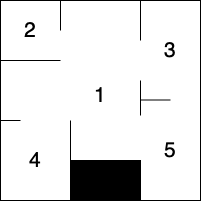
\includegraphics[width=2in]{figure/Map.drawio.png} 
		 \caption{Example of space layout} 
		 \label{fig:examplespace} 
\end{figure}
In Table~\ref{cont} we first have the singular context $[S]^{\gamma , \mathsf{LS}}$. Here the context would be one of the numbered rooms and $S$ would exist in that room. Note that $S$ can be an empty process, in other words, a context does not require a system to be present to exist. We can also see that each context has an environment, just like the systems. $\gamma$ stores the local variables and the physical space representation and $\mathsf{LS}$ stores the local channels. In the semantics we will see how this environment influences the systems present in the context. A context can also be a parallel composition of contexts, these parallel compositions allow for representing a full physical space, without the need for specified relations. For non-continuous, or discrete, space, this can be helpful as we do not have to keep track of the relations between contexts as their relation will no change, but they still exist in parallel. As our example has no defined continuous spaces, here the spaces would exist in parallel.
\\
The other two contexts define the relations between contexts. For this we have two different options, namely the externally connected relation $\mathsf{EC}(C_1, C_2)^{\gamma , \mathsf{LS}}$, this relation argues that systems from 1 context could move to the other context and depending on the specified model, could also communicate between the contexts. Relating it to \ref{fig:examplespace}, we would have $\mathsf{EC}(1,2)$  for example, as space 1 is directly connected to space 2. The environment of this context is a union of the environment of $C_1$ and $C_2$. The opposite of externally connected is disconnected $\mathsf{DC}(C_1, C_2)^{\gamma , \mathsf{LS}}$. As we do not allow for movements to non-externally connected contexts, disconnected contexts limit the possible actions which can be taken. The environment is again a combination of both contexts, and for continuous contexts could be used for moving closer to eventually allow for the exchanging of processes. In relation to \ref{fig:examplespace}, this would be $\mathsf{DC}(2,4)$. We would most likely not define this relation for discrete physical spaces like these rooms, as just saying they exist in parallel also argues that they cannot directly exchange processes.
\\
For our context semantics, to distinguish them from the other transition levels, we will use $\xRightarrow[]{}$ for context level transitions. We will use the transition label $\mu (S, E)$ to model movements, where $S$ is the system which moves and $E$ an expression which can be concretized to a destination context.
\begin{table}[H]
\normalsize
\centering
\begin{flalign*}
    \texttt{Out }&\frac{}{[\langle \gamma _S, \mathsf{LS}_S\rangle : S]^{\gamma _C, \mathsf{LS}_C} \xRightarrow[]{\mu (S, C')}[\quad]^{\gamma _C', \mathsf{LS}_C}} & & &\\
    \texttt{In } &\frac{}{[\quad]^{\gamma _C, \mathsf{LS}_C} \xRightarrow[]{\mu (S, C)}[\langle \gamma _S \cup \gamma _C, \mathsf{LS}_S \cup \mathsf{LS} _C \rangle : S']^{\gamma _C', \mathsf{LS}_C}} & & &\\
   \texttt{LPOut }&\frac{}{[\langle \gamma _{S_1}, \mathsf{LS}_{S_1}\rangle : S_1\ ||\ \langle \gamma _{S_2}, \mathsf{LS}_{S_2}\rangle : S_2]^{\gamma _C, \mathsf{LS}_C} \xRightarrow[]{\mu (S_1, E)}[\langle \gamma _{S_2}, \mathsf{LS}_{S_2}\rangle : S_2]^{\gamma _C', \mathsf{LS}_C}} & & &\\
     \texttt{RPOut }&\frac{}{[\langle \gamma _{S_1}, \mathsf{LS}_{S_1}\rangle : S_1\ ||\ \langle \gamma _{S_2}, \mathsf{LS}_{S_2}\rangle : S_2]^{\gamma _C, \mathsf{LS}_C} \xRightarrow[]{\mu (S_2, E)}[\langle \gamma _{S_1}, \mathsf{LS}_{S_1}\rangle : S_1]^{\gamma _C', \mathsf{LS}_C}} & & &\\
%    \texttt{LPIn } &\frac{}{[\langle \gamma _{S_2}, \mathsf{LS}_{S_2}\rangle : S_2]^{\gamma _C, \mathsf{LS}_C} \xRightarrow[]{\mu (S_1, C)}[\langle \gamma _{S_1} \cup \gamma _C, \mathsf{LS}_{S_1'} \cup \mathsf{LS} _C \rangle : S_1'\ ||\ \langle \gamma _{S_2}, \mathsf{LS}_{S_2}\rangle : S_2]^{\gamma _C', \mathsf{LS}_C}} & & &\\
        \texttt{RPIn } &\frac{}{[\langle \gamma _{S_1}, \mathsf{LS}_{S_1}\rangle : S_1]^{\gamma _C, \mathsf{LS}_C} \xRightarrow[]{\mu (S_2, C)}[\langle \gamma _{S_1}, \mathsf{LS}_{S_1}\rangle : S_1\ ||\ \langle \gamma _{S_2} \cup \gamma _C, \mathsf{LS}_{S_2} \cup \mathsf{LS} _C \rangle : S']^{\gamma _C', \mathsf{LS}_C}} & & &\\
    \texttt{LMov }&\frac{EC(C_1, C_2)}{[\langle \gamma _S, \mathsf{LS} _S \rangle : S]_1^{\gamma _{C_1}, \mathsf{LS}_{C_1}} \ || \ [\quad]_2^{\gamma _{C_2}, \mathsf{LS}_{C_2}} \xRightarrow[]{\mu (S, C_2)} [\quad]_1^{\gamma _{C_1}, \mathsf{LS}_{C_1}} \ || \ [\langle (\gamma _S \setminus \gamma _{C_1})\cup \gamma _{C_2}, (\mathsf{LS} _S \setminus \mathsf{LS} _{C_1}) \cup \mathsf{LS} _{C_2} \rangle : S']_2^{\gamma _{C_2}, \mathsf{LS}_{C_2}}} & & &\\
    \texttt{RMov }&\frac{EC(C_1, C_2)}{[\quad]_1^{\gamma _{C_1}, \mathsf{LS}_{C_1}} \ || \ [\langle \gamma _S, \mathsf{LS} _S \rangle : S]_2^{\gamma _{C_2}, \mathsf{LS}_{C_2}} \xRightarrow[]{\mu (S, C_1)} [\langle (\gamma _S \setminus \gamma _{C_2})\cup \gamma _{C_1}, (\mathsf{LS} _S \setminus \mathsf{LS} _{C_2}) \cup \mathsf{LS} _{C_1} \rangle : S']_1^{\gamma _{C_1}, \mathsf{LS}_{C_1}} \ || \ [\quad]_2^{\gamma _{C_2}, \mathsf{LS}_{C_2}}} & & &\\
%    \texttt{Con }&\frac{}{[S_1]_1^{\gamma _{C_1}, \mathsf{LS}_{C_1}} \ || \ [S_2]_2^{\gamma _{C_2}, \mathsf{LS}_{C_2}} \xRightarrow[]{\mathsf{EC}(C_1, C_2)} [S_1\ ||\ S_2 ]^{\gamma _{C_1} \cup \gamma _{C_2}, \mathsf{LS}_{C_1} \cup \mathsf{LS} _{C_2}}} & & &\\
%    \texttt{Dis }&\frac{}{[S_1\ ||\ S_2 ]^{\gamma _{C_1} \cup \gamma _{C_2}, \mathsf{LS}_{C_1} \cup \mathsf{LS} _{C_2}} \xRightarrow[]{\mathsf{DC}(C_1, C_2)} [S_1]_1^{\gamma _{C_1}, \mathsf{LS}_{C_1}} \ || \ [S_2]_2^{\gamma _{C_2}, \mathsf{LS}_{C_2}}} & & &\\
\end{flalign*}
\caption{The system level semantics.}
\label{opsem4}
\end{table}




% RESULTS
% % CREATED BY DAVID FRISK, 2016
\chapter{Theoretical correctness}
We will first go over some essential lemmas, to prove certain behavior of our system. The proofs of these lemmas can be found in the appendix.\\
Given 2 systems $S_1$ and $S_2$ proof:\\
\begin{lemma}
    \begin{enumerate}
    \item $S_1 \ || \ S_2 \equiv S_2\ ||\ S_1$
    \item $(S_1 \ ||\ S_2 )\ || \ S_3 \equiv S_1 \ ||\ (S_2 \ || \ S_3)$
    \item $S_1 \ || \ \Gamma : 0 \equiv S_1$
\end{enumerate}
\end{lemma}
\begin{lemma}
Lemma 2 is regarding the non-blocking behavior of broadcasted messages.\\ 
$ch=* \land S_1 \xrightarrow[]{\pi !(\Tilde{v})^{ch}}S_1' \implies S_1\ ||\ S_2 \xrightarrow[]{\pi !(\Tilde{v})^{ch}}S_1'\ ||\ S_2'\quad $ for any $S_2$.\\
\end{lemma}

\begin{lemma}
    Lemma 3 shows the blocking of multi cast channels.\\
$ch\not = * \land S_1 \xrightarrow[]{\pi !(\Tilde{v})^{ch}}S_1' \implies S_1\ ||\ S_2 \xrightarrow[]{\pi !(\Tilde{v})^{ch}}S_1'\ ||\ S_2'\quad$ for any $S_2$ such that:
\begin{enumerate}
    \item $ch \in \mathsf{LS} \land S_2 \xrightarrow[]{\pi ?(\Tilde{v})^{ch}}S_2'$\\
    $\lor$
    \item $ch \not \in \mathsf{LS}$
\end{enumerate}
\end{lemma}

\begin{lemma}
    This lemma is about the blocking of unicast, to show it should never go unanswered\\
$S_1 \xrightarrow[]{\Pi \mathsf{G} (\Tilde{v})^{ch}} S_1' \implies S_1 \ || \ S_2 \xrightarrow[]{\tau} S_1' \ || \ S_2'$ for any $S_2$ such that $S_2 \xrightarrow[]{\Pi \mathsf{S} (\Tilde{v})^{ch}} S_2'$. 
\end{lemma}




% CONCLUSION
% CREATED BY DAVID FRISK, 2016
\chapter{Conclusion}

You may consider to instead divide this chapter into discussion of the results and a summary. 

\section{Discussion}

\section{Conclusion}


% REFERENCES / BIBLIOGRAPHY
\cleardoublepage
\phantomsection % So hyperref does not link to the section above
\addcontentsline{toc}{chapter}{Bibliography}
\printbibliography

% APPENDICES
\cleardoublepage
\appendix
\setcounter{page}{1}
\pagenumbering{Roman}			% Capitalized roman numbering starting from I (one)

% CREATED BY DAVID FRISK, 2016
\chapter{Appendix 1}
\section{Lemma 1}
\begin{lemma}
    \begin{enumerate}
    \item $S_1 \ || \ S_2 \equiv S_2\ ||\ S_1$
    \item $(S_1 \ ||\ S_2 )\ || \ S_3 \equiv S_1 \ ||\ (S_2 \ || \ S_3)$
    \item $S_1 \ || \ \Gamma : 0 \equiv S_1$
\end{enumerate}
\end{lemma}
We will proof this lemma by case analysis on $\alpha$. We will have 5 cases with multiple subcases each. To proof a case we need to find a matching transition on both sides which are possible by the semantic rules. Only when all cases and subcases have been covered have we proven the statement.\\
\textbf{1. }The first point is proving commutativity. We can see in the syntax that the cases we have to cover are: $\Pi ! (\Tilde{v})^{ch}$, $\Pi ? (\Tilde{v})^{ch}$, $ \Pi \mathsf{G}(\Tilde{v})^{ch}$, $ \Pi \mathsf{S}(\Tilde{v})^{ch}$ and $ \tau$\\
\textbf{Case 1: } Consider $\alpha = \Pi ! (\Tilde{v})^{ch}$.\\
\indent \textbf{Subcase 1.1: }$S_1 \ || \ S_2 \xrightarrow[]{\alpha} S_1' \ || \ S_2'$. Assume $S_1\not= S_1'$ and $S_2\not= S_2'$, as those cases are covered by subcases 1.2, 1.3 and 1.4. This transition then has two subcases of its own.\\
\indent \indent \textbf{Subcase 1.1.1: } Consider \texttt{Lpar}, we have $S_1 \xrightarrow[]{\Pi ! (\Tilde{v})^{ch}} S_1' $ and $ S_2 \xrightarrow[]{\Pi ? (\Tilde{v})^{ch}} S_2'$. Giving us $S_1 \ || \ S_2 \xrightarrow[]{\Pi ! (\Tilde{v})^{ch}} S_1 ' \ || \ S_2'$. By \texttt{Rpar} on $S_2\ ||\ S_1$, we also get $ S_2 \xrightarrow[]{\Pi ? (\Tilde{v})^{ch}} S_2'$ and $S_1 \xrightarrow[]{\Pi ! (\Tilde{v})^{ch}} S_1' $, resulting in $S_2 \ || \ S_1 \xrightarrow[]{\Pi ! (\Tilde{v})^{ch}} S_2 ' \ || \ S_1'$. Showing $S_1 \ || \ S_2 \equiv S_2\ ||\ S_1$.\\
\indent \indent \textbf{Subcase 1.1.2: } Consider \texttt{Rpar}, we have $S_1 \xrightarrow[]{\Pi ? (\Tilde{v})^{ch}} S_1' $ and $ S_2 \xrightarrow[]{\Pi ! (\Tilde{v})^{ch}} S_2'$. Giving us $S_1 \ || \ S_2 \xrightarrow[]{\Pi ! (\Tilde{v})^{ch}} S_1 ' \ || \ S_2'$. By \texttt{Lpar} on $S_2\ ||\ S_1$, we also get $ S_2 \xrightarrow[]{\Pi ! (\Tilde{v})^{ch}} S_2'$ and $S_1 \xrightarrow[]{\Pi ? (\Tilde{v})^{ch}} S_1' $, resulting in $S_2 \ || \ S_1 \xrightarrow[]{\Pi ! (\Tilde{v})^{ch}} S_2 ' \ || \ S_1'$. Showing $S_1 \ || \ S_2 \equiv S_2\ ||\ S_1$.\\
\indent \textbf{Subcase 1.2: }$S_1 \ || \ S_2 \xrightarrow[]{\alpha} S_1' \ || \ S_2$. In this case only $S_1$ transitions. Looking at the semantics, it does not immediately seem like such a transition exists. However, by \texttt{Nsys} we can discard the $S \xrightarrow[]{\Pi ? (\Tilde{v})^{ch}} S'$ transition making it $\langle \gamma , \mathsf{LS} \rangle : P \xmapsto[]{\widetilde{\Pi ? (\Tilde{v})^{ch}}} \langle \gamma , \mathsf{LS} \rangle : P$.\\ 
\indent \indent \textbf{Subcase 1.2.1: } Consider \texttt{Lpar}, we get $S_1 \xrightarrow[]{\Pi ! (\Tilde{v})^{ch}} S_1' $ and $ S_2 \xrightarrow[]{\Pi ? (\Tilde{v})^{ch}} S_2'$, but for this case by \texttt{Nsys}, we get $S_2=\langle \gamma , \mathsf{LS} \rangle : P$ and $\langle \gamma , \mathsf{LS} \rangle : P  \xmapsto[]{\widetilde{\Pi ? (\Tilde{v})^{ch}}} \langle \gamma , \mathsf{LS} \rangle : P$. This results in $S_1 \ || \ S_2 \xrightarrow[]{\Pi ! (\Tilde{v})^{ch}} S_1' \ || \ S_2$. By \texttt{Rpar} and \texttt{Nsys}, we then get $\langle \gamma , \mathsf{LS} \rangle : P \xmapsto[]{\widetilde{\Pi ? (\Tilde{v})^{ch}}} \langle \gamma , \mathsf{LS} \rangle : P$ for $S_2=\langle \gamma , \mathsf{LS} \rangle : P$ and $S_1 \xrightarrow[]{\Pi ! (\Tilde{v})^{ch}} S_1' $ as well. This results in $S_2 \ || \ S_1 \xrightarrow[]{\Pi ! (\Tilde{v})^{ch}} S_2 \ || \ S_1'$. Showing $S_1 \ || \ S_2 \equiv S_2\ ||\ S_1$.\\
\indent \indent \textbf{Subcase 1.2.2: } Consider \texttt{Rpar}, we would get $S_2$ with the sending transition, but by our IH, we have that $S_2$ does not transition. By \texttt{Nsys}, we see that it is only possible for the receiving, and thus this is not possible.\\
\indent \textbf{Subcase 1.3: }$S_1 \ || \ S_2 \xrightarrow[]{\alpha} S_1 \ || \ S_2'$. In this case we have the opposite of the previous case.\\
\indent \indent \textbf{Subcase 1.3.1: } Consider \texttt{Lpar}, just like in case 1.2.2, this is not possible, because $S_1$ would be the sending system, but we know $S_1$ does not transition.\\
\indent \indent \textbf{Subcase 1.3.2: } Consider \texttt{Rpar}, we would get $S_1 \xrightarrow[]{\Pi ? (\Tilde{v})^{ch}} S_1' $ and $ S_2 \xrightarrow[]{\Pi ! (\Tilde{v})^{ch}} S_2'$, but for this case by \texttt{Nsys}, we get $S_1=\langle \gamma , \mathsf{LS} \rangle : P$ and $\langle \gamma , \mathsf{LS} \rangle : P \xmapsto[]{\widetilde{\Pi ? (\Tilde{v})^{ch}}} \langle \gamma , \mathsf{LS} \rangle : P$. This results in $S_1 \ || \ S_2 \xrightarrow[]{\Pi ! (\Tilde{v})^{ch}} S_1 \ || \ S_2'$. By \texttt{Lpar} and \texttt{Nsys}, we then also get $S_2 \xrightarrow[]{\Pi ! (\Tilde{v})^{ch}} S_2'$ and $\langle \gamma , \mathsf{LS} \rangle : P \xmapsto[]{\widetilde{\Pi ? (\Tilde{v})^{ch}}} \langle \gamma , \mathsf{LS} \rangle : P$ with $S_1=\langle \gamma , \mathsf{LS} \rangle : P$ for $S_2 \ || \ S_1$. This results in $S_2 \ || \ S_1 \xrightarrow[]{\Pi ! (\Tilde{v})^{ch}} S_2 \ || \ S_1'$. Showing $S_1 \ || \ S_2 \equiv S_2\ ||\ S_1$.\\
\indent \textbf{Subcase 1.4:} $S_1 \ || \ S_2 \xrightarrow[]{\alpha} S_1 \ || \ S_2$, this case is a combination of subcases 1.2.2 and 1.3.1. We have explained why for a send transition, at least one system has to transition. This means this transition is not possible.\\
\\
\textbf{Case 2: } Consider $\alpha = \Pi ? (\Tilde{v})^{ch}$.\\
\indent \textbf{Subcase 2.1: }$S_1 \ || \ S_2 \xrightarrow[]{\alpha} S_1' \ || \ S_2'$. Assume $S_1\not= S_1'$ and $S_2\not= S_2'$, as those cases are covered by subcases 1.2, 1.3 and 1.4. Consider \texttt{Prec}, we get $S_1 \xrightarrow[]{\Pi ? (\Tilde{v})^{ch}} S_1' $ and $ S_2 \xrightarrow[]{\Pi ? (\Tilde{v})^{ch}} S_2'$. By \texttt{Prec}, we also get $ S_2 \xrightarrow[]{\Pi ? (\Tilde{v})^{ch}} S_2'$ and $S_1 \xrightarrow[]{\Pi ? (\Tilde{v})^{ch}} S_1' $ for $S_2\ ||\ S_1$, showing $S_1 \ || \ S_2 \equiv S_2\ ||\ S_1$.\\
\indent \textbf{Subcase 2.2: }$S_1 \ || \ S_2 \xrightarrow[]{\alpha} S_1' \ || \ S_2$. In this case only $S_1$ transitions. By \texttt{Nsys} we can discard the $S \xrightarrow[]{\Pi ? (\Tilde{v})^{ch}} S'$ transition making it $\langle \gamma , \mathsf{LS} \rangle : P \xmapsto[]{\widetilde{\Pi ? (\Tilde{v})^{ch}}} \langle \gamma , \mathsf{LS} \rangle : P$. Consider \texttt{Prec}, we get $S_1 \xrightarrow[]{\Pi ? (\Tilde{v})^{ch}} S_1' $ and $ S_2 \xrightarrow[]{\Pi ? (\Tilde{v})^{ch}} S_2'$, by \texttt{Nsys} on $S_2=\langle \gamma , \mathsf{LS} \rangle : P$, we get $\langle \gamma , \mathsf{LS} \rangle : P  \xmapsto[]{\widetilde{\Pi ? (\Tilde{v})^{ch}}} \langle \gamma , \mathsf{LS} \rangle : P$. This results in $S_1 \ || \ S_2 \xrightarrow[]{\Pi ? (\Tilde{v})^{ch}} S_1' \ || \ S_2$. By \texttt{Prec} and \texttt{Nsys} on $S_2$, we also get $S_2 \ || \ S_1 \xrightarrow[]{\Pi ? (\Tilde{v})^{ch}} S_2 \ || \ S_1'$ for $S_2\ ||\ S_1$, showing $S_1 \ || \ S_2 \equiv S_2\ ||\ S_1$.\\ 
\indent \textbf{Subcase 2.3: }$S_1 \ || \ S_2 \xrightarrow[]{\alpha} S_1 \ || \ S_2'$. In this case we have the opposite of the previous case. Consider \texttt{Prec}, we get $S_1 \xrightarrow[]{\Pi ? (\Tilde{v})^{ch}} S_1' $ and $ S_2 \xrightarrow[]{\Pi ? (\Tilde{v})^{ch}} S_2'$, by \texttt{Nsys} on $S_1=\langle \gamma , \mathsf{LS} \rangle : P$, we get $\langle \gamma , \mathsf{LS} \rangle : P  \xmapsto[]{\widetilde{\Pi ? (\Tilde{v})^{ch}}} \langle \gamma , \mathsf{LS} \rangle : P$. This results in $S_1 \ || \ S_2 \xrightarrow[]{\Pi ? (\Tilde{v})^{ch}} S_1 \ || \ S_2'$. By \texttt{Prec} and \texttt{Nsys} on $S_1$, we also get $S_2 \ || \ S_1 \xrightarrow[]{\Pi ? (\Tilde{v})^{ch}} S_2' \ || \ S_1$ for $S_2\ ||\ S_1$, showing $S_1 \ || \ S_2 \equiv S_2\ ||\ S_1$.\\
\indent \textbf{Subcase 2.4:} $S_1 \ || \ S_2 \xrightarrow[]{\alpha} S_1 \ || \ S_2$. This is a combination of subcase 2.2 and 2.3. Consider \texttt{Prec}, we get $S_1 \xrightarrow[]{\Pi ? (\Tilde{v})^{ch}} S_1' $ and $ S_2 \xrightarrow[]{\Pi ? (\Tilde{v})^{ch}} S_2'$. By \texttt{Nsys} on $S_1=\langle \gamma , \mathsf{LS} \rangle : P_1$ and $S_2=\langle \gamma , \mathsf{LS} \rangle : P_2$, we get $\langle \gamma , \mathsf{LS} \rangle : P_1  \xmapsto[]{\widetilde{\Pi ? (\Tilde{v})^{ch}}} \langle \gamma , \mathsf{LS} \rangle : P_1$ and $\langle \gamma , \mathsf{LS} \rangle : P_2  \xmapsto[]{\widetilde{\Pi ? (\Tilde{v})^{ch}}} \langle \gamma , \mathsf{LS} \rangle : P_2$. This gives us $S_1 \ || \ S_2 \xrightarrow[]{\Pi ? (\Tilde{v})^{ch}} S_1 \ || \ S_2$. By \texttt{Prec} and \texttt{Nsys} on both $S_2$ and $S_1$, we also get $S_2 \ || \ S_1 \xrightarrow[]{\Pi ? (\Tilde{v})^{ch}} S_2' \ || \ S_1$ for $S_2\ ||\ S_1$, showing $S_1 \ || \ S_2 \equiv S_2\ ||\ S_1$.\\
\\
\textbf{Case 3: } Consider $\alpha = \Pi \mathsf{G}(\Tilde{v})^{ch}$.\\
\indent \textbf{Subcase 3.1: }$S_1 \ || \ S_2 \xrightarrow[]{\alpha} S_1' \ || \ S_2'$. Assume $S_1\not= S_1'$ and $S_2\not= S_2'$, as those cases are covered by subcases 1.2, 1.3 and 1.4. The rules which have $\Pi \mathsf{G}(\Tilde{v})^{ch}$ exposed are \texttt{Lget} and \texttt{Rget}. Each of these only transition one of the systems, while the other stays in the same state. This means it is not possible for $S_1\not= S_1'$ and $S_2\not= S_2'$. This makes sense, as only a single process can ask to get information at a time, just like only 1 send transition can be send at a time. If the second system also transitions, this would have to be by supplying information, however this would result in a hidden, $\tau$, transition. Therefore this case is not possible.\\
\indent \textbf{Subcase 3.2: }$S_1 \ || \ S_2 \xrightarrow[]{\alpha} S_1' \ || \ S_2$. In this case only $S_1$ transitions. \\
\indent \indent \textbf{Subcase 3.2.1: } Consider \texttt{Lget}, we get $S_1 \xrightarrow[]{\Pi \mathsf{G}(\Tilde{v})^{ch}} S_1'$, resulting in $S_1 \ || \ S_2 \xrightarrow[]{\Pi \mathsf{G}(\Tilde{v})^{ch}} S_1' \ || \ S_2$. By \texttt{Rget} on $S_2\ ||\ S_1$, we also get $S_1 \xrightarrow[]{\Pi \mathsf{G}(\Tilde{v})^{ch}} S_1'$, resulting in $S_2 \ || \ S_1 \xrightarrow[]{\Pi \mathsf{G}(\Tilde{v})^{ch}} S_2 \ || \ S_1'$, showing $S_1 \ || \ S_2 \equiv S_2\ ||\ S_1$ in this case.\\ 
\indent \indent \textbf{Subcase 3.2.2: } Consider \texttt{Rget}, this would require $S_2$ to transition, but we know it does not. So this subcase is not possible.\\
\indent \textbf{Subcase 3.3: }$S_1 \ || \ S_2 \xrightarrow[]{\alpha} S_1 \ || \ S_2'$. In this case we have the opposite of the previous case.\\
\indent \indent \textbf{Subcase 3.2.1: } Consider \texttt{Lget}, this would require $S_2$ to transition, but we know it does not. So this subcase is not possible.\\ 
\indent \indent \textbf{Subcase 3.2.2: } Consider \texttt{Rget}, we get $S_2 \xrightarrow[]{\Pi \mathsf{G}(\Tilde{v})^{ch}} S_2'$, resulting in $S_1 \ || \ S_2 \xrightarrow[]{\Pi \mathsf{G}(\Tilde{v})^{ch}} S_1 \ || \ S_2'$. By \texttt{Lget} on $S_2\ ||\ S_1$, we also get $S_2 \xrightarrow[]{\Pi \mathsf{G}(\Tilde{v})^{ch}} S_2'$, resulting in $S_2 \ || \ S_1 \xrightarrow[]{\Pi \mathsf{G}(\Tilde{v})^{ch}} S_2' \ || \ S_1$, showing $S_1 \ || \ S_2 \equiv S_2\ ||\ S_1$ in this case.\\
\indent \textbf{Subcase 3.4:} $S_1 \ || \ S_2 \xrightarrow[]{\alpha} S_1 \ || \ S_2$. Consider \texttt{Nsys}, is states the only transition which can be discarded is the send transition. As that is not our $\alpha$, this case is not possible.\\
\\
\textbf{Case 4: } Consider $\alpha = \Pi \mathsf{S}(\Tilde{v})^{ch}$.\\
\indent \textbf{Subcase 4.1: }$S_1 \ || \ S_2 \xrightarrow[]{\alpha} S_1' \ || \ S_2'$. Assume $S_1\not= S_1'$ and $S_2\not= S_2'$, as those cases are covered by subcases 1.2, 1.3 and 1.4. Just like in subcase 3.1, this case is not possible. Only 1 system can supply at a time, meaning we cannot have two systems transition with an exposed supply transition. \\
\indent \textbf{Subcase 4.2: }$S_1 \ || \ S_2 \xrightarrow[]{\alpha} S_1' \ || \ S_2$. In this case only $S_1$ transitions. \\ 
\indent \indent \textbf{Subcase 4.2.1: } Consider \texttt{Lsup}, we get $S_1 \xrightarrow[]{\Pi \mathsf{S}(\Tilde{v})^{ch}} S_1'$, resulting in $S_1 \ || \ S_2 \xrightarrow[]{\Pi \mathsf{S}(\Tilde{v})^{ch}} S_1' \ || \ S_2$. By \texttt{Rsup} on $S_2\ ||\ S_1$, we also get $S_1 \xrightarrow[]{\Pi \mathsf{S}(\Tilde{v})^{ch}} S_1'$, resulting in $S_2 \ || \ S_1 \xrightarrow[]{\Pi \mathsf{S}(\Tilde{v})^{ch}} S_2 \ || \ S_1'$, showing $S_1 \ || \ S_2 \equiv S_2\ ||\ S_1$ in this case.\\
\indent \indent \textbf{Subcase 4.2.2: } Consider \texttt{Rsup}, this would require $S_2$ to transition, but we know it does not. So this subcase is not possible.\\
\indent \textbf{Subcase 4.3: }$S_1 \ || \ S_2 \xrightarrow[]{\alpha} S_1 \ || \ S_2'$. In this case we have the opposite of the previous case.\\
\indent \indent \textbf{Subcase 4.3.1: } Consider \texttt{Lsup}, this would require $S_2$ to transition, but we know it does not. So this subcase is not possible.\\
\indent \indent \textbf{Subcase 4.3.2: } Consider \texttt{Rsup}, we get $S_2 \xrightarrow[]{\Pi \mathsf{S}(\Tilde{v})^{ch}} S_2'$, resulting in $S_1 \ || \ S_2 \xrightarrow[]{\Pi \mathsf{S}(\Tilde{v})^{ch}} S_1 \ || \ S_2'$. By \texttt{Lsup} on $S_2\ ||\ S_1$, we also get $S_2 \xrightarrow[]{\Pi \mathsf{S}(\Tilde{v})^{ch}} S_2'$, resulting in $S_2 \ || \ S_1 \xrightarrow[]{\Pi \mathsf{S}(\Tilde{v})^{ch}} S_2' \ || \ S_1$, showing $S_1 \ || \ S_2 \equiv S_2\ ||\ S_1$ in this case.\\
\indent \textbf{Subcase 4.4:} $S_1 \ || \ S_2 \xrightarrow[]{\alpha} S_1 \ || \ S_2$. Consider \texttt{Nsys}, is states the only transition which can be discarded is the send transition. As that is not our $\alpha$, this case is not possible.\\
\\
\textbf{Case 5: } Consider $\alpha = \tau$.\\
\indent \textbf{Subcase 5.1: }$S_1 \ || \ S_2 \xrightarrow[]{\alpha} S_1' \ || \ S_2'$. Assume $S_1\not= S_1'$ and $S_2\not= S_2'$, as those cases are covered by subcases 1.2, 1.3 and 1.4. This leaves us with 2 subcases, as \texttt{Ltau} and \texttt{Rtau} only have 1 system transitioning.\\
\indent \indent \textbf{Subcase 5.1.1: } Consider \texttt{Luni}, we get $S_1 \xrightarrow[]{\Pi \mathsf{G}(\Tilde{v})^{ch}} S_1'$ and $S_2 \xrightarrow[]{\Pi \mathsf{S}(\Tilde{v})^{ch}} S_2'$ resulting in $S_1 \ || \ S_2 \xrightarrow[]{\tau} S_1' \ || \ S_2'$. By \texttt{Runi}, we also get $S_2 \xrightarrow[]{\Pi \mathsf{S}(\Tilde{v})^{ch}} S_2'$ and $S_1 \xrightarrow[]{\Pi \mathsf{G}(\Tilde{v})^{ch}} S_1'$ for $S_2\ ||\ S_1$. Resulting in $S_2 \ || \ S_1 \xrightarrow[]{\tau} S_2' \ || \ S_1'$. Therefore $S_1 \ || \ S_2 \equiv S_2\ ||\ S_1$ holds for this case.\\
\indent \indent \textbf{Subcase 5.1.2: } Consider \texttt{Runi}, we get $S_1 \xrightarrow[]{\Pi \mathsf{S}(\Tilde{v})^{ch}} S_1'$ and $S_2 \xrightarrow[]{\Pi \mathsf{G}(\Tilde{v})^{ch}} S_2'$ resulting in $S_1 \ || \ S_2 \xrightarrow[]{\tau} S_1' \ || \ S_2'$. By \texttt{Luni}, we also get $S_2 \xrightarrow[]{\Pi \mathsf{G}(\Tilde{v})^{ch}} S_2'$ and $S_1 \xrightarrow[]{\Pi \mathsf{S}(\Tilde{v})^{ch}} S_1'$ for $S_2\ ||\ S_1$. Resulting in $S_2 \ || \ S_1 \xrightarrow[]{\tau} S_2' \ || \ S_1'$. Therefore $S_1 \ || \ S_2 \equiv S_2\ ||\ S_1$ holds for this case.\\
\indent \textbf{Subcase 5.2: }$S_1 \ || \ S_2 \xrightarrow[]{\alpha} S_1' \ || \ S_2$. In this case only $S_1$ transitions with $\tau$. Three of the $\tau$-transition rules do not allow this, because by \texttt{Nsys} we cannot discard the transition. The rules \texttt{Luni}, \texttt{Runi} and \texttt{Rtau} require $S_2$ to transition, which for our subcase is not the case. This leaves us with one more case. Consider \texttt{Ltau}, we get $S_1 \xrightarrow[]{\tau} S_1'$ resulting in $S_1 \ || \ S_2 \xrightarrow[]{\tau} S_1' \ || \ S_2$. By \texttt{Rtau}, also $S_2\ ||\ S_1$ gives us $S_1 \xrightarrow[]{\tau} S_1'$ and $S_2 \ || \ S_1 \xrightarrow[]{\tau} S_2 \ || \ S_1'$. Meaning $S_1 \ || \ S_2 \equiv S_2\ ||\ S_1$ holds for this case.\\ 
\indent \textbf{Subcase 5.3: }$S_1 \ || \ S_2 \xrightarrow[]{\alpha} S_1 \ || \ S_2'$. In this case we have the opposite of the previous case. Once again we have 3 transitions which are not possible, namely \texttt{Luni}, \texttt{Runi} and \texttt{Ltau}. Consider \texttt{Rtau}, we get $S_2 \xrightarrow[]{\tau} S_2'$ resulting in $S_1 \ || \ S_2 \xrightarrow[]{\tau} S_1 \ || \ S_2'$. By \texttt{Ltau}, also $S_2\ ||\ S_1$ gives us $S_2 \xrightarrow[]{\tau} S_2'$ and $S_2 \ || \ S_1 \xrightarrow[]{\tau} S_2' \ || \ S_1$. Meaning $S_1 \ || \ S_2 \equiv S_2\ ||\ S_1$ holds for this case.\\
\indent \textbf{Subcase 5.4:} $S_1 \ || \ S_2 \xrightarrow[]{\alpha} S_1 \ || \ S_2$. This case is not possible, for a $\tau$, transition to happen, we need at least 1 system to make that transition as by \texttt{Nsys}, this is not possible to discard.\\
As it holds for all cases, we have proven commutativity. $\square$
\\
\textbf{2. }We have shown commutativity and the next point is associativity, $(S_1 \ ||\ S_2 )\ || \ S_3 \equiv S_1 \ ||\ (S_2 \ || \ S_3)$. We will once again perform a case analysis to prove this. Because our rules only deal with parallel compositions of 2 systems, we will consider the two systems between parentheses as 1. By our grammer, we can then consider the possible other rules and match those.\\
\textbf{Case 1: } Consider $\alpha = \Pi ! (\Tilde{v})^{ch}$.\\
\indent \textbf{Subcase 1.1: }$(S_1 \ || \ S_2)\ ||\ S_3 \xrightarrow[]{\alpha} (S_1' \ || \ S_2')\ ||\ S_3'$. Assume $S_i\not = S_i'$ as that is covered by other subcases. As we have a sending transition, we will end up with 3 subcases, namely of each system being the sending system, because only 1 system can send at a time.\\
\indent \indent \textbf{Subcase 1.1.1: } Consider \texttt{Lpar}, we get $S_1 \ || \ S_2 \xrightarrow[]{\Pi ! (\Tilde{v})^{ch}} S_1' \ || \ S_2'$ and $S_3 \xrightarrow[]{\Pi ? (\Tilde{v})^{ch}} S_3'$. We can now split the first transition into two subcases, one where $S_1$ is sending and one where $S_2$ is sending.\\
\indent \indent \indent \textbf{Subcase 1.1.1.1: } Consider \texttt{Lpar} on $S_1\ ||\ S_2$. We get $S_1 \xrightarrow[]{\Pi ! (\Tilde{v})^{ch}} S_1'$ and $S_2 \xrightarrow[]{\Pi ? (\Tilde{v})^{ch}} S_2'$, together with $S_3 \xrightarrow[]{\Pi ? (\Tilde{v})^{ch}} S_3'$, we then have $(S_1 \ || \ S_2)\ ||\ S_3 \xrightarrow[]{\Pi ! (\Tilde{v})^{ch}} (S_1' \ || \ S_2')\ ||\ S_3'$. By \texttt{Lpar} on $S_1 \ ||\ (S_2 \ || \ S_3)$, we get $S_1 \xrightarrow[]{\Pi ! (\Tilde{v})^{ch}} S_1'$ and $S_2 \ || \ S_3 \xrightarrow[]{\Pi ? (\Tilde{v})^{ch}} S_2' \ || \ S_3'$. By \texttt{Prec}, we then get $S_2 \xrightarrow[]{\Pi ? (\Tilde{v})^{ch}} S_2'$ and $S_3 \xrightarrow[]{\Pi ? (\Tilde{v})^{ch}} S_3'$, which are the same transitions and shows $(S_1 \ ||\ S_2 )\ || \ S_3 \equiv S_1 \ ||\ (S_2 \ || \ S_3)$ for this case.\\
\indent \indent \indent \textbf{Subcase 1.1.1.2: } Now consider \texttt{Rpar} on $S_1\ ||\ S_2$. We get $S_1 \xrightarrow[]{\Pi ? (\Tilde{v})^{ch}} S_1'$ and $S_2 \xrightarrow[]{\Pi ! (\Tilde{v})^{ch}} S_2'$, together with $S_3 \xrightarrow[]{\Pi ? (\Tilde{v})^{ch}} S_3'$, we then have $(S_1 \ || \ S_2)\ ||\ S_3 \xrightarrow[]{\Pi ! (\Tilde{v})^{ch}} (S_1' \ || \ S_2')\ ||\ S_3'$. By \texttt{Rpar} on $S_1 \ ||\ (S_2 \ || \ S_3)$, we get $S_1 \xrightarrow[]{\Pi ? (\Tilde{v})^{ch}} S_1'$ and $S_2 \ || \ S_3 \xrightarrow[]{\Pi ! (\Tilde{v})^{ch}} S_2' \ || \ S_3'$. By \texttt{Lpar}, we then get $S_2 \xrightarrow[]{\Pi ! (\Tilde{v})^{ch}} S_2'$ and $S_3 \xrightarrow[]{\Pi ? (\Tilde{v})^{ch}} S_3'$, which are the same transitions and shows $(S_1 \ ||\ S_2 )\ || \ S_3 \equiv S_1 \ ||\ (S_2 \ || \ S_3)$ for this case.\\
\indent \indent \textbf{Subcase 1.1.2: } Consider \texttt{Rpar}, we get $S_1 \ || \ S_2 \xrightarrow[]{\Pi ? (\Tilde{v})^{ch}} S_1' \ || \ S_2'$ and $S_3 \xrightarrow[]{\Pi ! (\Tilde{v})^{ch}} S_3'$. By \texttt{Prec} on $S_1\ ||\ S_2$, we then get $S_1 \xrightarrow[]{\Pi ? (\Tilde{v})^{ch}} S_1'$ and $S_2 \xrightarrow[]{\Pi ? (\Tilde{v})^{ch}} S_2'$. By \texttt{Rpar} on $S_1 \ ||\ (S_2 \ || \ S_3)$, we get $S_1 \xrightarrow[]{\Pi ? (\Tilde{v})^{ch}} S_1'$ and $S_2 \ || \ S_3 \xrightarrow[]{\Pi ! (\Tilde{v})^{ch}} S_2' \ || \ S_3'$. By \texttt{Rpar} on $S_2\ ||\ S_3$, we then get $S_2 \xrightarrow[]{\Pi ? (\Tilde{v})^{ch}} S_2'$ and $S_3 \xrightarrow[]{\Pi ! (\Tilde{v})^{ch}} S_3'$, which are the same transitions and shows $(S_1 \ ||\ S_2 )\ || \ S_3 \equiv S_1 \ ||\ (S_2 \ || \ S_3)$ for this case.\\
\indent \textbf{Subcase 1.2: }$(S_1 \ || \ S_2)\ ||\ S_3 \xrightarrow[]{\alpha} (S_1' \ || \ S_2)\ ||\ S_3$. Here only $S_1$ transitions. From the commutativity proof, we know that for our $\alpha$, the sending transition, the sending system has to transition. This means our sending transition has to be $S_1$.\\
\indent \indent \textbf{Subcase 1.2.1: } Consider \texttt{Lpar}, we get $S_1 \ || \ S_2 \xrightarrow[]{\Pi ! (\Tilde{v})^{ch}} S_1' \ || \ S_2'$ and $S_3 \xrightarrow[]{\Pi ? (\Tilde{v})^{ch}} S_3'$.\\
\indent \indent \indent \textbf{Subcase 1.2.1.1: } Consider \texttt{Lpar} on $S_1\ ||\ S_2$. We get $S_1 \xrightarrow[]{\Pi ! (\Tilde{v})^{ch}} S_1'$ and $S_2 \xrightarrow[]{\Pi ? (\Tilde{v})^{ch}} S_2'$. By \texttt{Nsys} on $S_2 \xrightarrow[]{\Pi ? (\Tilde{v})^{ch}} S_2'$ and $S_3 \xrightarrow[]{\Pi ? (\Tilde{v})^{ch}} S_3'$, we get $S_2 \xrightarrow[]{\Pi ? (\Tilde{v})^{ch}} S_2$ and $S_3 \xrightarrow[]{\Pi ? (\Tilde{v})^{ch}} S_3$. We then have $(S_1 \ || \ S_2)\ ||\ S_3 \xrightarrow[]{\Pi ! (\Tilde{v})^{ch}} (S_1' \ || \ S_2)\ ||\ S_3$. By \texttt{Lpar} on $S_1 \ ||\ (S_2 \ || \ S_3)$, we get $S_1 \xrightarrow[]{\Pi ! (\Tilde{v})^{ch}} S_1'$ and $S_2 \ || \ S_3 \xrightarrow[]{\Pi ? (\Tilde{v})^{ch}} S_2' \ || \ S_3'$. By \texttt{Prec} and \texttt{Nsys} on both transitions, we then get $S_2 \xrightarrow[]{\Pi ? (\Tilde{v})^{ch}} S_2$ and $S_3 \xrightarrow[]{\Pi ? (\Tilde{v})^{ch}} S_3$, which are the same transitions and shows $(S_1 \ ||\ S_2 )\ || \ S_3 \equiv S_1 \ ||\ (S_2 \ || \ S_3)$ for this case. \\
\indent \indent \indent \textbf{Subcase 1.2.1.1: } Consider \texttt{Rpar} on $S_1 \ || \ S_2 \xrightarrow[]{\Pi ! (\Tilde{v})^{ch}} S_1' \ || \ S_2'$. This would require $S_2$ to be the sending system, however we know $S_2$ does not transition and thus this is not possible.\\
\indent \indent \textbf{Subcase 1.2.2: } Consider \texttt{Rpar}. This would require $S_3$ to be the sending system, however we know $S_3$ does not transition and thus this is not possible.\\
\indent \textbf{Subcase 1.3: }$(S_1 \ || \ S_2)\ ||\ S_3 \xrightarrow[]{\alpha} (S_1 \ || \ S_2')\ ||\ S_3$. This case is similar to the previous subcase, but this time we have $S_2$ which has to be the sending transition.\\
\indent \indent \textbf{Subcase 1.3.1: } Consider \texttt{Lpar}, we get $S_1 \ || \ S_2 \xrightarrow[]{\Pi ! (\Tilde{v})^{ch}} S_1' \ || \ S_2'$ and $S_3 \xrightarrow[]{\Pi ? (\Tilde{v})^{ch}} S_3'$.\\
\indent \indent \indent \textbf{Subcase 1.3.1.1: } Consider \texttt{Lpar} on $S_1 \ || \ S_2 \xrightarrow[]{\Pi ! (\Tilde{v})^{ch}} S_1' \ || \ S_2'$. This would require $S_1$ to be the sending system, however we know $S_1$ does not transition and thus this is not possible.\\
\indent \indent \indent \textbf{Subcase 1.3.1.2: } Consider \texttt{Rpar} on $S_1\ ||\ S_2$. We get $S_1 \xrightarrow[]{\Pi ? (\Tilde{v})^{ch}} S_1'$ and $S_2 \xrightarrow[]{\Pi ! (\Tilde{v})^{ch}} S_2'$. By \texttt{Nsys} on $S_1 \xrightarrow[]{\Pi ? (\Tilde{v})^{ch}} S_1'$ and $S_3 \xrightarrow[]{\Pi ? (\Tilde{v})^{ch}} S_3'$, we get $S_1 \xrightarrow[]{\Pi ? (\Tilde{v})^{ch}} S_1$ and $S_3 \xrightarrow[]{\Pi ? (\Tilde{v})^{ch}} S_3$. We then have $(S_1 \ || \ S_2)\ ||\ S_3 \xrightarrow[]{\Pi ! (\Tilde{v})^{ch}} (S_1 \ || \ S_2')\ ||\ S_3$. By \texttt{Rpar} on $S_1 \ ||\ (S_2 \ || \ S_3)$, we get $S_1 \xrightarrow[]{\Pi ? (\Tilde{v})^{ch}} S_1'$ and $S_2 \ || \ S_3 \xrightarrow[]{\Pi ! (\Tilde{v})^{ch}} S_2' \ || \ S_3'$. By \texttt{Lpar} and \texttt{Nsys} on $S_3$, we then get $S_2 \xrightarrow[]{\Pi ! (\Tilde{v})^{ch}} S_2'$ and $S_3 \xrightarrow[]{\Pi ? (\Tilde{v})^{ch}} S_3$, which are the same transitions and shows $(S_1 \ ||\ S_2 )\ || \ S_3 \equiv S_1 \ ||\ (S_2 \ || \ S_3)$ for this case.\\
\indent \indent \textbf{Subcase 1.3.2: } Consider \texttt{Rpar}. This would require $S_3$ to be the sending system, however we know $S_3$ does not transition and thus this is not possible.\\
\indent \textbf{Subcase 1.4: }$(S_1 \ || \ S_2)\ ||\ S_3 \xrightarrow[]{\alpha} (S_1 \ || \ S_2)\ ||\ S_3'$. This is once again a similar case, but this time with $S_3$ being the sending transition.\\
\indent \indent \textbf{Subcase 1.4.1: } Consider \texttt{Lpar}. This would require $S_1$ or $S_2$ to be the sending system, however we know neither transitions and thus this is not possible.\\
\indent \indent \textbf{Subcase 1.4.2: } Consider \texttt{Rpar}, we get $S_1 \ || \ S_2 \xrightarrow[]{\Pi ? (\Tilde{v})^{ch}} S_1' \ || \ S_2'$ and $S_3 \xrightarrow[]{\Pi ! (\Tilde{v})^{ch}} S_3'$. Now consider \texttt{Prec} on $S_1\ ||\ S_2$, we get $S_1 \xrightarrow[]{\Pi ? (\Tilde{v})^{ch}} S_1'$ and $S_2 \xrightarrow[]{\Pi ? (\Tilde{v})^{ch}} S_2'$. By \texttt{Nsys} on $S_1 \xrightarrow[]{\Pi ? (\Tilde{v})^{ch}} S_1'$ and $S_2 \xrightarrow[]{\Pi ? (\Tilde{v})^{ch}} S_2'$, we get $S_1 \xrightarrow[]{\Pi ? (\Tilde{v})^{ch}} S_1$ and $S_2 \xrightarrow[]{\Pi ? (\Tilde{v})^{ch}} S_2$. Resulting in $(S_1 \ || \ S_2)\ ||\ S_3 \xrightarrow[]{\Pi ! (\Tilde{v})^{ch}} (S_1 \ || \ S_2)\ ||\ S_3' $. By \texttt{Rpar} on $S_1 \ ||\ (S_2 \ || \ S_3)$ we get $S_1 \xrightarrow[]{\Pi ? (\Tilde{v})^{ch}} S_1'$ and $S_2 \ || \ S_3 \xrightarrow[]{\Pi ! (\Tilde{v})^{ch}} S_2' \ || \ S_3'$. Then by \texttt{Rpar} again on the latter transition we get $S_2 \xrightarrow[]{\Pi ? (\Tilde{v})^{ch}} S_2'$ and $S_3 \xrightarrow[]{\Pi ! (\Tilde{v})^{ch}} S_3'$. Resulting in $(S_1 \ || \ S_2)\ ||\ S_3 \xrightarrow[]{\Pi ! (\Tilde{v})^{ch}} (S_1 \ || \ S_2)\ ||\ S_3' $ with the same transitions. Showing $(S_1 \ ||\ S_2 )\ || \ S_3 \equiv S_1 \ ||\ (S_2 \ || \ S_3)$ for this case.\\
\indent \textbf{Subcase 1.5: }$(S_1 \ || \ S_2)\ ||\ S_3 \xrightarrow[]{\alpha} (S_1' \ || \ S_2')\ ||\ S_3$. In this case $S_1$ and $S_2$ transition, meaning either of them can be the sending system.\\
\indent \indent \textbf{Subcase 1.5.1: } Consider \texttt{Lpar}, we get $S_1 \ || \ S_2 \xrightarrow[]{\Pi ! (\Tilde{v})^{ch}} S_1' \ || \ S_2'$ and $S_3 \xrightarrow[]{\Pi ? (\Tilde{v})^{ch}} S_3'$.\\
\indent \indent \indent \textbf{Subcase 1.5.1.1: } Consider \texttt{Lpar} on $S_1\ ||\ S_2$. We get $S_1 \xrightarrow[]{\Pi ! (\Tilde{v})^{ch}} S_1'$ and $S_2 \xrightarrow[]{\Pi ? (\Tilde{v})^{ch}} S_2'$. By \texttt{Nsys} on $S_3 \xrightarrow[]{\Pi ? (\Tilde{v})^{ch}} S_3'$, we get $S_3 \xrightarrow[]{\Pi ? (\Tilde{v})^{ch}} S_3$, we then have $(S_1 \ || \ S_2)\ ||\ S_3 \xrightarrow[]{\Pi ! (\Tilde{v})^{ch}} (S_1' \ || \ S_2')\ ||\ S_3$. By \texttt{Lpar} on $S_1 \ ||\ (S_2 \ || \ S_3)$, we get $S_1 \xrightarrow[]{\Pi ! (\Tilde{v})^{ch}} S_1'$ and $S_2 \ || \ S_3 \xrightarrow[]{\Pi ? (\Tilde{v})^{ch}} S_2' \ || \ S_3'$. By \texttt{Prec}, we then get $S_2 \xrightarrow[]{\Pi ? (\Tilde{v})^{ch}} S_2'$ and $S_3 \xrightarrow[]{\Pi ? (\Tilde{v})^{ch}} S_3'$ and by \texttt{Nsys} on the latter we get $S_3 \xrightarrow[]{\Pi ? (\Tilde{v})^{ch}} S_3$, which are the same transitions and shows $(S_1 \ ||\ S_2 )\ || \ S_3 \equiv S_1 \ ||\ (S_2 \ || \ S_3)$ for this case.\\
\indent \indent \indent \textbf{Subcase 1.5.1.2: } Now consider \texttt{Rpar} on $S_1\ ||\ S_2$. We get $S_1 \xrightarrow[]{\Pi ? (\Tilde{v})^{ch}} S_1'$ and $S_2 \xrightarrow[]{\Pi ! (\Tilde{v})^{ch}} S_2'$. By \texttt{Nsys} on $S_3 \xrightarrow[]{\Pi ? (\Tilde{v})^{ch}} S_3'$, we get $S_3 \xrightarrow[]{\Pi ? (\Tilde{v})^{ch}} S_3$, we then have $(S_1 \ || \ S_2)\ ||\ S_3 \xrightarrow[]{\Pi ! (\Tilde{v})^{ch}} (S_1' \ || \ S_2')\ ||\ S_3$. By \texttt{Rpar} on $S_1 \ ||\ (S_2 \ || \ S_3)$, we get $S_1 \xrightarrow[]{\Pi ? (\Tilde{v})^{ch}} S_1'$ and $S_2 \ || \ S_3 \xrightarrow[]{\Pi ! (\Tilde{v})^{ch}} S_2' \ || \ S_3'$. By \texttt{Lpar}, we then get $S_2 \xrightarrow[]{\Pi ! (\Tilde{v})^{ch}} S_2'$ and $S_3 \xrightarrow[]{\Pi ? (\Tilde{v})^{ch}} S_3'$, and by \texttt{Nsys} we have $S_3 \xrightarrow[]{\Pi ? (\Tilde{v})^{ch}} S_3$, which are the same transitions and shows $(S_1 \ ||\ S_2 )\ || \ S_3 \equiv S_1 \ ||\ (S_2 \ || \ S_3)$ for this case.\\
\indent \indent \textbf{Subcase 1.5.2: } Consider \texttt{Rpar}, this would require $S_3$ to be the sending system, but as it does not transition this is not possible.\\
\indent \textbf{Subcase 1.6: }$(S_1 \ || \ S_2)\ ||\ S_3 \xrightarrow[]{\alpha} (S_1' \ || \ S_2)\ ||\ S_3'$. This is similar to the previous case, but now with $S_1$ or $S_3$ being the sending transition.\\
\indent \indent \textbf{Subcase 1.6.1: } Consider \texttt{Lpar}, we get $S_1 \ || \ S_2 \xrightarrow[]{\Pi ! (\Tilde{v})^{ch}} S_1' \ || \ S_2'$ and $S_3 \xrightarrow[]{\Pi ? (\Tilde{v})^{ch}} S_3'$.\\
\indent \indent \indent \textbf{Subcase 1.6.1.1: } Consider \texttt{Lpar} on $S_1\ ||\ S_2$. We get $S_1 \xrightarrow[]{\Pi ! (\Tilde{v})^{ch}} S_1'$ and $S_2 \xrightarrow[]{\Pi ? (\Tilde{v})^{ch}} S_2'$. By \texttt{Nsys} on $S_2 \xrightarrow[]{\Pi ? (\Tilde{v})^{ch}} S_2'$, we get $S_2 \xrightarrow[]{\Pi ? (\Tilde{v})^{ch}} S_2$. Together with $S_3 \xrightarrow[]{\Pi ? (\Tilde{v})^{ch}} S_3'$ we then have $(S_1 \ || \ S_2)\ ||\ S_3 \xrightarrow[]{\Pi ! (\Tilde{v})^{ch}} (S_1' \ || \ S_2)\ ||\ S_3'$. By \texttt{Lpar} on $S_1 \ ||\ (S_2 \ || \ S_3)$, we get $S_1 \xrightarrow[]{\Pi ! (\Tilde{v})^{ch}} S_1'$ and $S_2 \ || \ S_3 \xrightarrow[]{\Pi ? (\Tilde{v})^{ch}} S_2' \ || \ S_3'$. By \texttt{Prec}, we then get $S_2 \xrightarrow[]{\Pi ? (\Tilde{v})^{ch}} S_2'$ and $S_3 \xrightarrow[]{\Pi ? (\Tilde{v})^{ch}} S_3'$ and by \texttt{Nsys} on the latter we get $S_2 \xrightarrow[]{\Pi ? (\Tilde{v})^{ch}} S_2$, which are the same transitions and shows $(S_1 \ ||\ S_2 )\ || \ S_3 \equiv S_1 \ ||\ (S_2 \ || \ S_3)$ for this case.\\
\indent \indent \indent \textbf{Subcase 1.6.1.2: } Consider \texttt{Rpar} on $S_1\ ||\ S_2$. This would require $S_2$ to be the sending transition but as it does not transition this is not possible.\\
\indent \indent \textbf{Subcase 1.6.2: } Consider \texttt{Rpar}, we get $S_1 \ || \ S_2 \xrightarrow[]{\Pi ? (\Tilde{v})^{ch}} S_1' \ || \ S_2'$ and $S_3 \xrightarrow[]{\Pi ! (\Tilde{v})^{ch}} S_3'$. By \texttt{Prec} on $S_1\ ||\ S_2$, we then get $S_1 \xrightarrow[]{\Pi ? (\Tilde{v})^{ch}} S_1'$ and $S_2 \xrightarrow[]{\Pi ? (\Tilde{v})^{ch}} S_2'$, combined with \texttt{Nsys} on the latter we get $S_2 \xrightarrow[]{\Pi ? (\Tilde{v})^{ch}} S_2$. Resulting in $(S_1 \ || \ S_2)\ ||\ S_3 \xrightarrow[]{\Pi ! (\Tilde{v})^{ch}} (S_1' \ || \ S_2)\ ||\ S_3'$. By \texttt{Rpar} on $S_1 \ ||\ (S_2 \ || \ S_3)$, we get $S_1 \xrightarrow[]{\Pi ? (\Tilde{v})^{ch}} S_1'$ and $S_2 \ || \ S_3 \xrightarrow[]{\Pi ! (\Tilde{v})^{ch}} S_2' \ || \ S_3'$. By \texttt{Rpar} on $S_2\ ||\ S_3$, we then get $S_2 \xrightarrow[]{\Pi ? (\Tilde{v})^{ch}} S_2'$ and $S_3 \xrightarrow[]{\Pi ! (\Tilde{v})^{ch}} S_3'$. By \texttt{Nsys} on $S_2 \xrightarrow[]{\Pi ? (\Tilde{v})^{ch}} S_2'$ we get $S_2 \xrightarrow[]{\Pi ? (\Tilde{v})^{ch}} S_2$, which are the same transitions and shows $(S_1 \ ||\ S_2 )\ || \ S_3 \equiv S_1 \ ||\ (S_2 \ || \ S_3)$ for this case.\\
\indent \textbf{Subcase 1.7: }$(S_1 \ || \ S_2)\ ||\ S_3 \xrightarrow[]{\alpha} (S_1 \ || \ S_2')\ ||\ S_3'$. Once again this is a similar case to the previous subcases but with $S_2$ or $S_3$ being the sending system.\\
\indent \indent \textbf{Subcase 1.7.1: } Consider \texttt{Lpar}, we get $S_1 \ || \ S_2 \xrightarrow[]{\Pi ! (\Tilde{v})^{ch}} S_1' \ || \ S_2'$ and $S_3 \xrightarrow[]{\Pi ? (\Tilde{v})^{ch}} S_3'$.\\
\indent \indent \indent \textbf{Subcase 1.7.1.1: } Consider \texttt{Lpar} on $S_1\ ||\ S_2$. This would require $S_1$ to be the sending transition but as it does not transition this is not possible.\\ 
\indent \indent \indent \textbf{Subcase 1.7.1.2: }Consider \texttt{Rpar} on $S_1\ ||\ S_2$. We get $S_1 \xrightarrow[]{\Pi ? (\Tilde{v})^{ch}} S_1'$ and $S_2 \xrightarrow[]{\Pi ! (\Tilde{v})^{ch}} S_2'$. By \texttt{Nsys} on $S_1 \xrightarrow[]{\Pi ? (\Tilde{v})^{ch}} S_1'$, we get $S_1 \xrightarrow[]{\Pi ? (\Tilde{v})^{ch}} S_1$. Together with $S_3 \xrightarrow[]{\Pi ? (\Tilde{v})^{ch}} S_3'$ we then have $(S_1 \ || \ S_2)\ ||\ S_3 \xrightarrow[]{\Pi ! (\Tilde{v})^{ch}} (S_1 \ || \ S_2')\ ||\ S_3'$. By \texttt{Rpar} on $S_1 \ ||\ (S_2 \ || \ S_3)$, we get $S_1 \xrightarrow[]{\Pi ? (\Tilde{v})^{ch}} S_1'$ and $S_2 \ || \ S_3 \xrightarrow[]{\Pi ! (\Tilde{v})^{ch}} S_2' \ || \ S_3'$. By \texttt{Rpar} again, we then get $S_2 \xrightarrow[]{\Pi ! (\Tilde{v})^{ch}} S_2'$ and $S_3 \xrightarrow[]{\Pi ? (\Tilde{v})^{ch}} S_3'$ and by \texttt{Nsys} on $S_1 \xrightarrow[]{\Pi ? (\Tilde{v})^{ch}} S_1'$ we get $S_1 \xrightarrow[]{\Pi ? (\Tilde{v})^{ch}} S_1$. These are the same transitions and shows $(S_1 \ ||\ S_2 )\ || \ S_3 \equiv S_1 \ ||\ (S_2 \ || \ S_3)$ for this case.\\
\indent \indent \textbf{Subcase 1.7.2: }  Consider \texttt{Rpar}, we get $S_1 \ || \ S_2 \xrightarrow[]{\Pi ? (\Tilde{v})^{ch}} S_1' \ || \ S_2'$ and $S_3 \xrightarrow[]{\Pi ! (\Tilde{v})^{ch}} S_3'$. By \texttt{Prec} on $S_1\ ||\ S_2$, we then get $S_1 \xrightarrow[]{\Pi ? (\Tilde{v})^{ch}} S_1'$ and $S_2 \xrightarrow[]{\Pi ? (\Tilde{v})^{ch}} S_2'$, combined with \texttt{Nsys} on the first we get $S_1 \xrightarrow[]{\Pi ? (\Tilde{v})^{ch}} S_1$. Resulting in $(S_1 \ || \ S_2)\ ||\ S_3 \xrightarrow[]{\Pi ! (\Tilde{v})^{ch}} (S_1 \ || \ S_2')\ ||\ S_3'$. By \texttt{Rpar} on $S_1 \ ||\ (S_2 \ || \ S_3)$, we get $S_1 \xrightarrow[]{\Pi ? (\Tilde{v})^{ch}} S_1'$ and $S_2 \ || \ S_3 \xrightarrow[]{\Pi ! (\Tilde{v})^{ch}} S_2' \ || \ S_3'$. By \texttt{Rpar} on $S_2\ ||\ S_3$, we then get $S_2 \xrightarrow[]{\Pi ? (\Tilde{v})^{ch}} S_2'$ and $S_3 \xrightarrow[]{\Pi ! (\Tilde{v})^{ch}} S_3'$. By \texttt{Nsys} on $S_1 \xrightarrow[]{\Pi ? (\Tilde{v})^{ch}} S_1'$ we get $S_1 \xrightarrow[]{\Pi ? (\Tilde{v})^{ch}} S_1$, which are the same transitions and shows $(S_1 \ ||\ S_2 )\ || \ S_3 \equiv S_1 \ ||\ (S_2 \ || \ S_3)$ for this case.\\
\indent \textbf{Subcase 1.8: }$(S_1 \ || \ S_2)\ ||\ S_3 \xrightarrow[]{\alpha} (S_1 \ || \ S_2)\ ||\ S_3$. As none of the systems transition, this case is not possible as for a sending action, a system has to transition.\\
\\
\textbf{Case 2: } Consider $\alpha = \Pi ? (\Tilde{v})^{ch}$.\\
\indent \textbf{Subcase 2.1: }$(S_1 \ || \ S_2)\ ||\ S_3 \xrightarrow[]{\alpha} (S_1' \ || \ S_2')\ ||\ S_3'$. Consider \texttt{Prec}, we get $S_1 \ || \ S_2 \xrightarrow[]{\Pi ? (\Tilde{v})^{ch}} S_1' \ || \ S_2'$ and $S_3 \xrightarrow[]{\Pi ? (\Tilde{v})^{ch}} S_3'$. By \texttt{Prec} again on $S_1 \ || \ S_2 \xrightarrow[]{\Pi ? (\Tilde{v})^{ch}} S_1' \ || \ S_2'$, we get $S_1 \xrightarrow[]{\Pi ? (\Tilde{v})^{ch}} S_1'$ and $S_2 \xrightarrow[]{\Pi ? (\Tilde{v})^{ch}} S_2'$. This gives us $(S_1 \ || \ S_2)\ ||\ S_3 \xrightarrow[]{\Pi ? (\Tilde{v})^{ch}} (S_1' \ || \ S_2')\ ||\ S_3'$. By \texttt{Prec} twice on $S_1 \ ||\ (S_2 \ || \ S_3)$, we also get $S_1 \xrightarrow[]{\Pi ? (\Tilde{v})^{ch}} S_1'$, $S_2 \xrightarrow[]{\Pi ? (\Tilde{v})^{ch}} S_2'$ and $S_3 \xrightarrow[]{\Pi ? (\Tilde{v})^{ch}} S_3'$, which are the same transitions and shows $(S_1 \ ||\ S_2 )\ || \ S_3 \equiv S_1 \ ||\ (S_2 \ || \ S_3)$ for this case.\\
\indent \textbf{Subcase 2.2: }$(S_1 \ || \ S_2)\ ||\ S_3 \xrightarrow[]{\alpha} (S_1' \ || \ S_2)\ ||\ S_3$. Consider \texttt{Prec}, we get $S_1 \ || \ S_2 \xrightarrow[]{\Pi ? (\Tilde{v})^{ch}} S_1' \ || \ S_2'$ and $S_3 \xrightarrow[]{\Pi ? (\Tilde{v})^{ch}} S_3'$. By \texttt{Prec} again on $S_1 \ || \ S_2 \xrightarrow[]{\Pi ? (\Tilde{v})^{ch}} S_1' \ || \ S_2'$, we get $S_1 \xrightarrow[]{\Pi ? (\Tilde{v})^{ch}} S_1'$ and $S_2 \xrightarrow[]{\Pi ? (\Tilde{v})^{ch}} S_2'$. By \texttt{Nsys} on $S_2$ and $S_3$ we get $S_2 \xrightarrow[]{\Pi ? (\Tilde{v})^{ch}} S_2$ and $S_3 \xrightarrow[]{\Pi ? (\Tilde{v})^{ch}} S_3$. This gives us $(S_1 \ || \ S_2)\ ||\ S_3 \xrightarrow[]{\Pi ? (\Tilde{v})^{ch}} (S_1' \ || \ S_2)\ ||\ S_3$. By \texttt{Prec} twice on $S_1 \ ||\ (S_2 \ || \ S_3)$ and \texttt{Nsys} on the resulting $S_2$ and $S_3$ transitions, we also get $S_1 \xrightarrow[]{\Pi ? (\Tilde{v})^{ch}} S_1'$, $S_2 \xrightarrow[]{\Pi ? (\Tilde{v})^{ch}} S_2$ and $S_3 \xrightarrow[]{\Pi ? (\Tilde{v})^{ch}} S_3$, which are the same transitions and shows $(S_1 \ ||\ S_2 )\ || \ S_3 \equiv S_1 \ ||\ (S_2 \ || \ S_3)$ for this case.\\
\indent \textbf{Subcase 2.3: }$(S_1 \ || \ S_2)\ ||\ S_3 \xrightarrow[]{\alpha} (S_1 \ || \ S_2')\ ||\ S_3$. Consider \texttt{Prec}, we get $S_1 \ || \ S_2 \xrightarrow[]{\Pi ? (\Tilde{v})^{ch}} S_1' \ || \ S_2'$ and $S_3 \xrightarrow[]{\Pi ? (\Tilde{v})^{ch}} S_3'$. By \texttt{Prec} again on $S_1 \ || \ S_2 \xrightarrow[]{\Pi ? (\Tilde{v})^{ch}} S_1' \ || \ S_2'$, we get $S_1 \xrightarrow[]{\Pi ? (\Tilde{v})^{ch}} S_1'$ and $S_2 \xrightarrow[]{\Pi ? (\Tilde{v})^{ch}} S_2'$. By \texttt{Nsys} on $S_1$ and $S_3$ we get $S_1 \xrightarrow[]{\Pi ? (\Tilde{v})^{ch}} S_1$ and $S_3 \xrightarrow[]{\Pi ? (\Tilde{v})^{ch}} S_3$. This gives us $(S_1 \ || \ S_2)\ ||\ S_3 \xrightarrow[]{\Pi ? (\Tilde{v})^{ch}} (S_1 \ || \ S_2')\ ||\ S_3$. By \texttt{Prec} twice on $S_1 \ ||\ (S_2 \ || \ S_3)$ and \texttt{Nsys} on the resulting $S_1$ and $S_3$ transitions, we also get $S_1 \xrightarrow[]{\Pi ? (\Tilde{v})^{ch}} S_1$, $S_2 \xrightarrow[]{\Pi ? (\Tilde{v})^{ch}} S_2'$ and $S_3 \xrightarrow[]{\Pi ? (\Tilde{v})^{ch}} S_3$, which are the same transitions and shows $(S_1 \ ||\ S_2 )\ || \ S_3 \equiv S_1 \ ||\ (S_2 \ || \ S_3)$ for this case.\\
\indent \textbf{Subcase 2.4: }$(S_1 \ || \ S_2)\ ||\ S_3 \xrightarrow[]{\alpha} (S_1 \ || \ S_2)\ ||\ S_3'$. Consider \texttt{Prec}, we get $S_1 \ || \ S_2 \xrightarrow[]{\Pi ? (\Tilde{v})^{ch}} S_1' \ || \ S_2'$ and $S_3 \xrightarrow[]{\Pi ? (\Tilde{v})^{ch}} S_3'$. By \texttt{Prec} again on $S_1 \ || \ S_2 \xrightarrow[]{\Pi ? (\Tilde{v})^{ch}} S_1' \ || \ S_2'$, we get $S_1 \xrightarrow[]{\Pi ? (\Tilde{v})^{ch}} S_1'$ and $S_2 \xrightarrow[]{\Pi ? (\Tilde{v})^{ch}} S_2'$. By \texttt{Nsys} on $S_1$ and $S_2$ we get $S_1 \xrightarrow[]{\Pi ? (\Tilde{v})^{ch}} S_1$ and $S_2 \xrightarrow[]{\Pi ? (\Tilde{v})^{ch}} S_2$. This gives us $(S_1 \ || \ S_2)\ ||\ S_3 \xrightarrow[]{\Pi ? (\Tilde{v})^{ch}} (S_1 \ || \ S_2)\ ||\ S_3'$. By \texttt{Prec} twice on $S_1 \ ||\ (S_2 \ || \ S_3)$ and \texttt{Nsys} on the resulting $S_1$ and $S_2$ transitions, we also get $S_1 \xrightarrow[]{\Pi ? (\Tilde{v})^{ch}} S_1$, $S_2 \xrightarrow[]{\Pi ? (\Tilde{v})^{ch}} S_2$ and $S_3 \xrightarrow[]{\Pi ? (\Tilde{v})^{ch}} S_3'$, which are the same transitions and shows $(S_1 \ ||\ S_2 )\ || \ S_3 \equiv S_1 \ ||\ (S_2 \ || \ S_3)$ for this case.\\
\indent \textbf{Subcase 2.5: }$(S_1 \ || \ S_2)\ ||\ S_3 \xrightarrow[]{\alpha} (S_1' \ || \ S_2')\ ||\ S_3$. Consider \texttt{Prec}, we get $S_1 \ || \ S_2 \xrightarrow[]{\Pi ? (\Tilde{v})^{ch}} S_1' \ || \ S_2'$ and $S_3 \xrightarrow[]{\Pi ? (\Tilde{v})^{ch}} S_3'$. By \texttt{Prec} again on $S_1 \ || \ S_2 \xrightarrow[]{\Pi ? (\Tilde{v})^{ch}} S_1' \ || \ S_2'$, we get $S_1 \xrightarrow[]{\Pi ? (\Tilde{v})^{ch}} S_1'$ and $S_2 \xrightarrow[]{\Pi ? (\Tilde{v})^{ch}} S_2'$. By \texttt{Nsys} on $S_3$ we get $S_3 \xrightarrow[]{\Pi ? (\Tilde{v})^{ch}} S_3$. This gives us $(S_1 \ || \ S_2)\ ||\ S_3 \xrightarrow[]{\Pi ? (\Tilde{v})^{ch}} (S_1' \ || \ S_2')\ ||\ S_3$. By \texttt{Prec} twice on $S_1 \ ||\ (S_2 \ || \ S_3)$ and \texttt{Nsys} on the resulting $S_3$ transition, we also get $S_1 \xrightarrow[]{\Pi ? (\Tilde{v})^{ch}} S_1'$, $S_2 \xrightarrow[]{\Pi ? (\Tilde{v})^{ch}} S_2'$ and $S_3 \xrightarrow[]{\Pi ? (\Tilde{v})^{ch}} S_3$, which are the same transitions and shows $(S_1 \ ||\ S_2 )\ || \ S_3 \equiv S_1 \ ||\ (S_2 \ || \ S_3)$ for this case.\\
\indent \textbf{Subcase 2.6: }$(S_1 \ || \ S_2)\ ||\ S_3 \xrightarrow[]{\alpha} (S_1' \ || \ S_2)\ ||\ S_3'$. Consider \texttt{Prec}, we get $S_1 \ || \ S_2 \xrightarrow[]{\Pi ? (\Tilde{v})^{ch}} S_1' \ || \ S_2'$ and $S_3 \xrightarrow[]{\Pi ? (\Tilde{v})^{ch}} S_3'$. By \texttt{Prec} again on $S_1 \ || \ S_2 \xrightarrow[]{\Pi ? (\Tilde{v})^{ch}} S_1' \ || \ S_2'$, we get $S_1 \xrightarrow[]{\Pi ? (\Tilde{v})^{ch}} S_1'$ and $S_2 \xrightarrow[]{\Pi ? (\Tilde{v})^{ch}} S_2'$. By \texttt{Nsys} on $S_2$ we get $S_2 \xrightarrow[]{\Pi ? (\Tilde{v})^{ch}} S_2$. This gives us $(S_1 \ || \ S_2)\ ||\ S_3 \xrightarrow[]{\Pi ? (\Tilde{v})^{ch}} (S_1' \ || \ S_2)\ ||\ S_3'$. By \texttt{Prec} twice on $S_1 \ ||\ (S_2 \ || \ S_3)$ and \texttt{Nsys} on the resulting $S_2$ transition, we also get $S_1 \xrightarrow[]{\Pi ? (\Tilde{v})^{ch}} S_1'$, $S_2 \xrightarrow[]{\Pi ? (\Tilde{v})^{ch}} S_2$ and $S_3 \xrightarrow[]{\Pi ? (\Tilde{v})^{ch}} S_3'$, which are the same transitions and shows $(S_1 \ ||\ S_2 )\ || \ S_3 \equiv S_1 \ ||\ (S_2 \ || \ S_3)$ for this case.\\
\indent \textbf{Subcase 2.7: }$(S_1 \ || \ S_2)\ ||\ S_3 \xrightarrow[]{\alpha} (S_1 \ || \ S_2')\ ||\ S_3'$. Consider \texttt{Prec}, we get $S_1 \ || \ S_2 \xrightarrow[]{\Pi ? (\Tilde{v})^{ch}} S_1' \ || \ S_2'$ and $S_3 \xrightarrow[]{\Pi ? (\Tilde{v})^{ch}} S_3'$. By \texttt{Prec} again on $S_1 \ || \ S_2 \xrightarrow[]{\Pi ? (\Tilde{v})^{ch}} S_1' \ || \ S_2'$, we get $S_1 \xrightarrow[]{\Pi ? (\Tilde{v})^{ch}} S_1'$ and $S_2 \xrightarrow[]{\Pi ? (\Tilde{v})^{ch}} S_2'$. By \texttt{Nsys} on $S_1$ we get $S_1 \xrightarrow[]{\Pi ? (\Tilde{v})^{ch}} S_1$. This gives us $(S_1 \ || \ S_2)\ ||\ S_3 \xrightarrow[]{\Pi ? (\Tilde{v})^{ch}} (S_1 \ || \ S_2')\ ||\ S_3'$. By \texttt{Prec} twice on $S_1 \ ||\ (S_2 \ || \ S_3)$ and \texttt{Nsys} on the resulting $S_1$ transition, we also get $S_1 \xrightarrow[]{\Pi ? (\Tilde{v})^{ch}} S_1$, $S_2 \xrightarrow[]{\Pi ? (\Tilde{v})^{ch}} S_2'$ and $S_3 \xrightarrow[]{\Pi ? (\Tilde{v})^{ch}} S_3'$, which are the same transitions and shows $(S_1 \ ||\ S_2 )\ || \ S_3 \equiv S_1 \ ||\ (S_2 \ || \ S_3)$ for this case.\\
\indent \textbf{Subcase 2.8: }$(S_1 \ || \ S_2)\ ||\ S_3 \xrightarrow[]{\alpha} (S_1 \ || \ S_2)\ ||\ S_3$. Consider \texttt{Prec}, we get $S_1 \ || \ S_2 \xrightarrow[]{\Pi ? (\Tilde{v})^{ch}} S_1' \ || \ S_2'$ and $S_3 \xrightarrow[]{\Pi ? (\Tilde{v})^{ch}} S_3'$. By \texttt{Prec} again on $S_1 \ || \ S_2 \xrightarrow[]{\Pi ? (\Tilde{v})^{ch}} S_1' \ || \ S_2'$, we get $S_1 \xrightarrow[]{\Pi ? (\Tilde{v})^{ch}} S_1'$ and $S_2 \xrightarrow[]{\Pi ? (\Tilde{v})^{ch}} S_2'$. By \texttt{Nsys} on all three transitions we get $S_1 \xrightarrow[]{\Pi ? (\Tilde{v})^{ch}} S_1$, $S_2 \xrightarrow[]{\Pi ? (\Tilde{v})^{ch}} S_2$ and $S_3 \xrightarrow[]{\Pi ? (\Tilde{v})^{ch}} S_3$. This gives us $(S_1 \ || \ S_2)\ ||\ S_3 \xrightarrow[]{\Pi ? (\Tilde{v})^{ch}} (S_1 \ || \ S_2)\ ||\ S_3$. By \texttt{Prec} twice on $S_1 \ ||\ (S_2 \ || \ S_3)$ and \texttt{Nsys} on the resulting transitions, we also get $S_1 \xrightarrow[]{\Pi ? (\Tilde{v})^{ch}} S_1$, $S_2 \xrightarrow[]{\Pi ? (\Tilde{v})^{ch}} S_2$ and $S_3 \xrightarrow[]{\Pi ? (\Tilde{v})^{ch}} S_3$, which are the same transitions and shows $(S_1 \ ||\ S_2 )\ || \ S_3 \equiv S_1 \ ||\ (S_2 \ || \ S_3)$ for this case.\\
\\
\textbf{Case 3: } Consider $\alpha = \Pi \mathsf{G}(\Tilde{v})^{ch}$.\\
\indent \textbf{Subcase 3.1: }$(S_1 \ || \ S_2)\ ||\ S_3 \xrightarrow[]{\alpha} (S_1' \ || \ S_2')\ ||\ S_3'$. We know only one system can send a get request at a time. We also know that if a system supplies, the transition is hidden, this means for this $\alpha$ only 1 system can transition and thus this subcase is not possible.\\
\indent \textbf{Subcase 3.2: }$(S_1 \ || \ S_2)\ ||\ S_3 \xrightarrow[]{\alpha} (S_1' \ || \ S_2)\ ||\ S_3$. As we know a system has to transition to send a get request, we know $S_1$ has to be the getting system. The only way to get this is by applying \texttt{Lget} twice. We get $S_1\xrightarrow[]{\Pi \mathsf{G}(\Tilde{v})^{ch}} S_1'$. By \texttt{Lget} on $S_1 \ ||\ (S_2 \ || \ S_3)$, we also get $S_1\xrightarrow[]{\Pi \mathsf{G}(\Tilde{v})^{ch}} S_1'$. which is the same transition and shows $(S_1 \ ||\ S_2 )\ || \ S_3 \equiv S_1 \ ||\ (S_2 \ || \ S_3)$ for this case.\\
\indent \textbf{Subcase 3.3: }$(S_1 \ || \ S_2)\ ||\ S_3 \xrightarrow[]{\alpha} (S_1 \ || \ S_2')\ ||\ S_3$. As we know a system has to transition to send a get request, we know $S_2$ has to be the getting system. The only way to get this is by applying \texttt{Lget} and \texttt{Rget}. We get $S_2\xrightarrow[]{\Pi \mathsf{G}(\Tilde{v})^{ch}} S_2'$. By \texttt{Rget} and \texttt{Lget} on $S_1 \ ||\ (S_2 \ || \ S_3)$, we also get $S_2\xrightarrow[]{\Pi \mathsf{G}(\Tilde{v})^{ch}} S_2'$. which is the same transition and shows $(S_1 \ ||\ S_2 )\ || \ S_3 \equiv S_1 \ ||\ (S_2 \ || \ S_3)$ for this case.\\
\indent \textbf{Subcase 3.4: }$(S_1 \ || \ S_2)\ ||\ S_3 \xrightarrow[]{\alpha} (S_1 \ || \ S_2)\ ||\ S_3'$. As we know a system has to transition to send a get request, we know $S_3$ has to be the getting system. The only way to get this is by applying \texttt{Rget}. We get $S_3\xrightarrow[]{\Pi \mathsf{G}(\Tilde{v})^{ch}} S_3'$. By \texttt{Rget} twice on $S_1 \ ||\ (S_2 \ || \ S_3)$, we also get $S_3\xrightarrow[]{\Pi \mathsf{G}(\Tilde{v})^{ch}} S_3'$. which is the same transition and shows $(S_1 \ ||\ S_2 )\ || \ S_3 \equiv S_1 \ ||\ (S_2 \ || \ S_3)$ for this case.\\
\indent \textbf{Subcase 3.5: }$(S_1 \ || \ S_2)\ ||\ S_3 \xrightarrow[]{\alpha} (S_1' \ || \ S_2')\ ||\ S_3$. We know only one system can send a get request at a time. We also know that if a system supplies, the transition is hidden, this means for this $\alpha$ only 1 system can transition and thus this subcase is not possible.\\
\indent \textbf{Subcase 3.6: }$(S_1 \ || \ S_2)\ ||\ S_3 \xrightarrow[]{\alpha} (S_1' \ || \ S_2)\ ||\ S_3'$. We know only one system can send a get request at a time. We also know that if a system supplies, the transition is hidden, this means for this $\alpha$ only 1 system can transition and thus this subcase is not possible.\\
\indent \textbf{Subcase 3.7: }$(S_1 \ || \ S_2)\ ||\ S_3 \xrightarrow[]{\alpha} (S_1 \ || \ S_2')\ ||\ S_3'$. We know only one system can send a get request at a time. We also know that if a system supplies, the transition is hidden, this means for this $\alpha$ only 1 system can transition and thus this subcase is not possible.\\
\indent \textbf{Subcase 3.8: }$(S_1 \ || \ S_2)\ ||\ S_3 \xrightarrow[]{\alpha} (S_1 \ || \ S_2)\ ||\ S_3$. We know by \texttt{Nsys}, that only a receive transition can be discarded. This means for our get transition, at least 1 system has to transition and thus this subcase is not possible.\\
\\
\textbf{Case 4: } Consider $\alpha = \Pi \mathsf{S}(\Tilde{v})^{ch}$.\\
\indent \textbf{Subcase 4.1: }$(S_1 \ || \ S_2)\ ||\ S_3 \xrightarrow[]{\alpha} (S_1' \ || \ S_2')\ ||\ S_3'$. This case has similar reasoning to the previous case. We know only one system can supply at a time. We also know that if a system in the same parallel composition has sent a get request, the transition is hidden, this means for this $\alpha$ only 1 system can transition and thus this subcase is not possible.\\
\indent \textbf{Subcase 4.2: }$(S_1 \ || \ S_2)\ ||\ S_3 \xrightarrow[]{\alpha} (S_1' \ || \ S_2)\ ||\ S_3$. As we know a system has to transition to supply, we know $S_1$ has to be the supplying system. The only way to get this is by applying \texttt{Lsup} twice. We get $S_1\xrightarrow[]{\Pi \mathsf{S}(\Tilde{v})^{ch}} S_1'$. By \texttt{Lsup} on $S_1 \ ||\ (S_2 \ || \ S_3)$, we also get $S_1\xrightarrow[]{\Pi \mathsf{S}(\Tilde{v})^{ch}} S_1'$. This is the same transition and shows $(S_1 \ ||\ S_2 )\ || \ S_3 \equiv S_1 \ ||\ (S_2 \ || \ S_3)$ for this case.\\
\indent \textbf{Subcase 4.3: }$(S_1 \ || \ S_2)\ ||\ S_3 \xrightarrow[]{\alpha} (S_1 \ || \ S_2')\ ||\ S_3$. As we know a system has to transition to supply, we know $S_2$ has to be the supplying system. The only way to get this is by applying \texttt{Lsup} and \texttt{Rsup}. We get $S_2\xrightarrow[]{\Pi \mathsf{S}(\Tilde{v})^{ch}} S_2'$. By \texttt{Rsup} and \texttt{Lsup} on $S_1 \ ||\ (S_2 \ || \ S_3)$, we also get $S_2\xrightarrow[]{\Pi \mathsf{S}(\Tilde{v})^{ch}} S_2'$. This is the same transition and shows $(S_1 \ ||\ S_2 )\ || \ S_3 \equiv S_1 \ ||\ (S_2 \ || \ S_3)$ for this case.\\
\indent \textbf{Subcase 4.4: }$(S_1 \ || \ S_2)\ ||\ S_3 \xrightarrow[]{\alpha} (S_1 \ || \ S_2)\ ||\ S_3'$. As we know a system has to transition to supply, we know $S_3$ has to be the supplying system. The only way to get this is by applying \texttt{Rsup}. We get $S_3\xrightarrow[]{\Pi \mathsf{S}(\Tilde{v})^{ch}} S_3'$. By \texttt{Rsup} twice on $S_1 \ ||\ (S_2 \ || \ S_3)$, we also get $S_3\xrightarrow[]{\Pi \mathsf{S}(\Tilde{v})^{ch}} S_3'$. This is the same transition and shows $(S_1 \ ||\ S_2 )\ || \ S_3 \equiv S_1 \ ||\ (S_2 \ || \ S_3)$ for this case.\\
\indent \textbf{Subcase 4.5: }$(S_1 \ || \ S_2)\ ||\ S_3 \xrightarrow[]{\alpha} (S_1' \ || \ S_2')\ ||\ S_3$. We know only one system can supply at a time. We also know that if a system in the same parallel composition has sent a get request, the transition is hidden, this means for this $\alpha$ only 1 system can transition and thus this subcase is not possible.\\
\indent \textbf{Subcase 4.6: }$(S_1 \ || \ S_2)\ ||\ S_3 \xrightarrow[]{\alpha} (S_1' \ || \ S_2)\ ||\ S_3'$. We know only one system can supply at a time. We also know that if a system in the same parallel composition has sent a get request, the transition is hidden, this means for this $\alpha$ only 1 system can transition and thus this subcase is not possible.\\
\indent \textbf{Subcase 4.7: }$(S_1 \ || \ S_2)\ ||\ S_3 \xrightarrow[]{\alpha} (S_1 \ || \ S_2')\ ||\ S_3'$. We know only one system can supply at a time. We also know that if a system in the same parallel composition has sent a get request, the transition is hidden, this means for this $\alpha$ only 1 system can transition and thus this subcase is not possible.\\
\indent \textbf{Subcase 4.8: }$(S_1 \ || \ S_2)\ ||\ S_3 \xrightarrow[]{\alpha} (S_1 \ || \ S_2)\ ||\ S_3$ We know by \texttt{Nsys}, that only a receive transition can be discarded. This means for our supply transition, at least 1 system has to transition and thus this subcase is not possible.\\
\\
\textbf{Case 5: } Consider $\alpha = \tau$.\\
\indent \textbf{Subcase 1.1: }$(S_1 \ || \ S_2)\ ||\ S_3 \xrightarrow[]{\alpha} (S_1' \ || \ S_2')\ ||\ S_3'$. For a $\tau$ transition, at most two systems can transition, the getting and the supplying one. As we have three systems transition for this subcase, this is not possible.\\
\indent \textbf{Subcase 5.2: }$(S_1 \ || \ S_2)\ ||\ S_3 \xrightarrow[]{\alpha} (S_1' \ || \ S_2)\ ||\ S_3$. For a $\tau$ transition, we need a get and a supply transition. As we only have one transitioning system, $S_1$, we know this one has to do both and thus we have a hidden transition. The only way this is possible is by \texttt{Ltau} twice. We get $S_1\xrightarrow[]{\tau} S_1'$, resulting in $(S_1 \ || \ S_2)\ ||\ S_3 \xrightarrow[]{\tau} (S_1' \ || \ S_2)\ ||\ S_3$. By \texttt{Ltau}, we also get $S_1\xrightarrow[]{\tau} S_1'$ for $S_1 \ ||\ (S_2 \ || \ S_3)$. This is the same transition and shows $(S_1 \ ||\ S_2 )\ || \ S_3 \equiv S_1 \ ||\ (S_2 \ || \ S_3)$ for this case.\\
\indent \textbf{Subcase 5.3: }$(S_1 \ || \ S_2)\ ||\ S_3 \xrightarrow[]{\alpha} (S_1 \ || \ S_2')\ ||\ S_3$. For a $\tau$ transition, we need a get and a supply transition. As we only have one transitioning system, $S_2$, we know this one has to do both and thus we have a hidden transition. The only way this is possible is by \texttt{Ltau} and \texttt{Rtau}. We get $S_2\xrightarrow[]{\tau} S_2'$, resulting in $(S_1 \ || \ S_2)\ ||\ S_3 \xrightarrow[]{\tau} (S_1 \ || \ S_2')\ ||\ S_3$. By \texttt{Rtau} and \texttt{Ltau}, we also get $S_2\xrightarrow[]{\tau} S_2'$ for $S_1 \ ||\ (S_2 \ || \ S_3)$. This is the same transition and shows $(S_1 \ ||\ S_2 )\ || \ S_3 \equiv S_1 \ ||\ (S_2 \ || \ S_3)$ for this case.\\
\indent \textbf{Subcase 5.4: }$(S_1 \ || \ S_2)\ ||\ S_3 \xrightarrow[]{\alpha} (S_1 \ || \ S_2)\ ||\ S_3'$. For a $\tau$ transition, we need a get and a supply transition. As we only have one transitioning system, $S_3$, we know this one has to do both and thus we have a hidden transition. The only way this is possible is by \texttt{Rtau}. We get $S_3\xrightarrow[]{\tau} S_3'$, resulting in $(S_1 \ || \ S_2)\ ||\ S_3 \xrightarrow[]{\tau} (S_1 \ || \ S_2)\ ||\ S_3'$. By \texttt{Rtau} twice, we also get $S_3\xrightarrow[]{\tau} S_3'$ for $S_1 \ ||\ (S_2 \ || \ S_3)$. This is the same transition and shows $(S_1 \ ||\ S_2 )\ || \ S_3 \equiv S_1 \ ||\ (S_2 \ || \ S_3)$ for this case.\\
\indent \textbf{Subcase 5.5: }$(S_1 \ || \ S_2)\ ||\ S_3 \xrightarrow[]{\alpha} (S_1' \ || \ S_2')\ ||\ S_3$. For a $\tau$ transition at most two systems can transition. One which send a get request and one which supplies. As we have two transitioning systems, $S_1$ and $S_2$, we know one has to supply and one has to get, giving us two subcases.\\
\indent \indent \textbf{Subcase 5.5.1: } Consider $S_1$ being the getting system, meaning $S_2$ supplies. Consider \texttt{Ltau} we get $S_1 \ || \ S_2 \xrightarrow[]{\tau} S_1' \ || \ S_2'$. By \texttt{Luni}, we then get $S_1\xrightarrow[]{\Pi \mathsf{G}(\Tilde{v})^{ch}} S_1'$ and $S_2\xrightarrow[]{\Pi \mathsf{S}(\Tilde{v})^{ch}} S_2'$, resulting in $(S_1 \ || \ S_2)\ ||\ S_3 \xrightarrow[]{\tau} (S_1' \ || \ S_2')\ ||\ S_3$. By \texttt{Luni} and \texttt{Lsup}, we also get $S_1\xrightarrow[]{\Pi \mathsf{G}(\Tilde{v})^{ch}} S_1'$ and $S_2\xrightarrow[]{\Pi \mathsf{S}(\Tilde{v})^{ch}} S_2'$ for $S_1 \ ||\ (S_2 \ || \ S_3)$. These are the same transitions and shows $(S_1 \ ||\ S_2 )\ || \ S_3 \equiv S_1 \ ||\ (S_2 \ || \ S_3)$ for this case.\\
\indent \indent \textbf{Subcase 5.5.2: } Consider $S_2$ being the getting system, meaning $S_1$ supplies. Consider \texttt{Ltau} we get $S_1 \ || \ S_2 \xrightarrow[]{\tau} S_1' \ || \ S_2'$. By \texttt{Runi}, we then get $S_1\xrightarrow[]{\Pi \mathsf{S}(\Tilde{v})^{ch}} S_1'$ and $S_2\xrightarrow[]{\Pi \mathsf{G}(\Tilde{v})^{ch}} S_2'$, resulting in $(S_1 \ || \ S_2)\ ||\ S_3 \xrightarrow[]{\tau} (S_1' \ || \ S_2')\ ||\ S_3$. By \texttt{Runi} and \texttt{Lget}, we also get $S_1\xrightarrow[]{\Pi \mathsf{S}(\Tilde{v})^{ch}} S_1'$ and $S_2\xrightarrow[]{\Pi \mathsf{G}(\Tilde{v})^{ch}} S_2'$ for $S_1 \ ||\ (S_2 \ || \ S_3)$. These are the same transitions and shows $(S_1 \ ||\ S_2 )\ || \ S_3 \equiv S_1 \ ||\ (S_2 \ || \ S_3)$ for this case.\\
\indent \textbf{Subcase 5.6: }$(S_1 \ || \ S_2)\ ||\ S_3 \xrightarrow[]{\alpha} (S_1' \ || \ S_2)\ ||\ S_3'$. For a $\tau$ transition at most two systems can transition. One which send a get request and one which supplies. As we have two transitioning systems, $S_1$ and $S_3$, we know one has to supply and one has to get, giving us two subcases.\\
\indent \indent \textbf{Subcase 5.6.1: } Consider $S_1$ being the getting system, meaning $S_3$ supplies. Consider \texttt{Luni} and \texttt{Lget} we get $S_1\xrightarrow[]{\Pi \mathsf{G}(\Tilde{v})^{ch}} S_1'$ and $S_3\xrightarrow[]{\Pi \mathsf{S}(\Tilde{v})^{ch}} S_3'$, resulting in $(S_1 \ || \ S_2)\ ||\ S_3 \xrightarrow[]{\tau} (S_1' \ || \ S_2)\ ||\ S_3'$. By \texttt{Luni} and \texttt{Rsup}, we also get $S_1\xrightarrow[]{\Pi \mathsf{G}(\Tilde{v})^{ch}} S_1'$ and $S_3\xrightarrow[]{\Pi \mathsf{S}(\Tilde{v})^{ch}} S_3'$ for $S_1 \ ||\ (S_2 \ || \ S_3)$. These are the same transitions and shows $(S_1 \ ||\ S_2 )\ || \ S_3 \equiv S_1 \ ||\ (S_2 \ || \ S_3)$ for this case.\\
\indent \indent \textbf{Subcase 5.6.2: } Consider $S_3$ being the getting system, meaning $S_1$ supplies. Consider \texttt{Runi} and \texttt{Lsup} we get $S_1\xrightarrow[]{\Pi \mathsf{S}(\Tilde{v})^{ch}} S_1'$ and $S_3\xrightarrow[]{\Pi \mathsf{G}(\Tilde{v})^{ch}} S_3'$, resulting in $(S_1 \ || \ S_2)\ ||\ S_3 \xrightarrow[]{\tau} (S_1' \ || \ S_2)\ ||\ S_3'$. By \texttt{Runi} and \texttt{Rget}, we also get $S_1\xrightarrow[]{\Pi \mathsf{S}(\Tilde{v})^{ch}} S_1'$ and $S_3\xrightarrow[]{\Pi \mathsf{G}(\Tilde{v})^{ch}} S_3'$ for $S_1 \ ||\ (S_2 \ || \ S_3)$. These are the same transitions and shows $(S_1 \ ||\ S_2 )\ || \ S_3 \equiv S_1 \ ||\ (S_2 \ || \ S_3)$ for this case.\\
\indent \textbf{Subcase 5.7: }$(S_1 \ || \ S_2)\ ||\ S_3 \xrightarrow[]{\alpha} (S_1 \ || \ S_2')\ ||\ S_3'$. For a $\tau$ transition at most two systems can transition. One which send a get request and one which supplies. As we have two transitioning systems, $S_2$ and $S_3$, we know one has to supply and one has to get, giving us two subcases.\\
\indent \indent \textbf{Subcase 5.7.1: } Consider $S_2$ being the getting system, meaning $S_3$ supplies. Consider \texttt{Luni} and \texttt{Rget} we get $S_2\xrightarrow[]{\Pi \mathsf{G}(\Tilde{v})^{ch}} S_2'$ and $S_3\xrightarrow[]{\Pi \mathsf{S}(\Tilde{v})^{ch}} S_3'$, resulting in $(S_1 \ || \ S_2)\ ||\ S_3 \xrightarrow[]{\tau} (S_1 \ || \ S_2')\ ||\ S_3'$. By \texttt{Rtau} and \texttt{Luni}, we also get $S_2\xrightarrow[]{\Pi \mathsf{G}(\Tilde{v})^{ch}} S_2'$ and $S_3\xrightarrow[]{\Pi \mathsf{S}(\Tilde{v})^{ch}} S_3'$ for $S_1 \ ||\ (S_2 \ || \ S_3)$. These are the same transitions and shows $(S_1 \ ||\ S_2 )\ || \ S_3 \equiv S_1 \ ||\ (S_2 \ || \ S_3)$ for this case.\\
\indent \indent \textbf{Subcase 5.7.2: } Consider $S_3$ being the getting system, meaning $S_2$ supplies. Consider \texttt{Runi} and \texttt{Rsup} we get $S_2\xrightarrow[]{\Pi \mathsf{S}(\Tilde{v})^{ch}} S_2'$ and $S_3\xrightarrow[]{\Pi \mathsf{G}(\Tilde{v})^{ch}} S_3'$, resulting in $(S_1 \ || \ S_2)\ ||\ S_3 \xrightarrow[]{\tau} (S_1 \ || \ S_2')\ ||\ S_3'$. By \texttt{Rtau} and \texttt{Runi}, we also get $S_2\xrightarrow[]{\Pi \mathsf{S}(\Tilde{v})^{ch}} S_2'$ and $S_3\xrightarrow[]{\Pi \mathsf{G}(\Tilde{v})^{ch}} S_3'$ for $S_1 \ ||\ (S_2 \ || \ S_3)$. These are the same transitions and shows $(S_1 \ ||\ S_2 )\ || \ S_3 \equiv S_1 \ ||\ (S_2 \ || \ S_3)$ for this case.\\
\indent \textbf{Subcase 5.8: }$(S_1 \ || \ S_2)\ ||\ S_3 \xrightarrow[]{\alpha} (S_1 \ || \ S_2)\ ||\ S_3$. For a $\tau$ transition, at least one system has to transition. As by \texttt{Nsys} only a receive transition can be discarded. Therefore this subcase is not possible.\\
\\
These cover all cases and therefore we have proven that associativity also holds. $\square$
\\
\textbf{3. }For the final point we want to show that a parallel composition with one of the processes being the empty process, acts the same as just the non-empty system. We will once again go by case analysis on $\alpha$. We know an empty process cannot do anything, besides discarding a receive transition as by \texttt{Nnul}. Besides the receiving transition, we cannot discard other transitions. The only possibilities are then $S_1$ performing the corresponding $\alpha$ transition.\\
\indent \textbf{Case 1: } Consider $\alpha = \Pi ! (\Tilde{v})^{ch}$.\\
\indent \indent \textbf{Subcase 1.1: } Consider \texttt{Lpar}, we get $S_1\xrightarrow[]{\Pi !(\Tilde{v})^{ch}} S_1'$. By \texttt{Sys} and our $\alpha$, we can also have that $S_1\xrightarrow[]{\Pi !(\Tilde{v})^{ch}} S_1'$ is the only possibility on the RHS.\\
\indent \indent \textbf{Subcase 1.2: } Consider \texttt{Rpar}, this would require the empty process to perform the sending action, which we know is not possible by \texttt{Nnul}.\\
\indent \textbf{Case 2: } Consider $\alpha = \Pi ? (\Tilde{v})^{ch}$.\\
\indent \indent \textbf{Subcase 2.1:} Consider \texttt{Prec}, we get $S_1\xrightarrow[]{\Pi ?(\Tilde{v})^{ch}} S_1'$ and together with \texttt{Nsys} and \texttt{Nnul} also $\Gamma : 0\xrightarrow[]{\Pi ?(\Tilde{v})^{ch}} \Gamma : 0$. By \texttt{Sys}, we also get $S_1\xrightarrow[]{\Pi ?(\Tilde{v})^{ch}} S_1'$ on the RHS.\\
\indent \indent \textbf{Subcase 2.2:} Consider \texttt{Prec}, we get $S_1\xrightarrow[]{\Pi ?(\Tilde{v})^{ch}} S_1'$ and together with \texttt{Nsys} on both this becomes $S_1\xrightarrow[]{\Pi ?(\Tilde{v})^{ch}} S_1$ and by \texttt{Nnul} also $\Gamma : 0\xrightarrow[]{\Pi ?(\Tilde{v})^{ch}} \Gamma : 0$. By \texttt{Nsys}, we also get $S_1\xrightarrow[]{\Pi ?(\Tilde{v})^{ch}} S_1$ on the RHS.\\
\indent \textbf{Case 3: } Consider $\alpha = \Pi \mathsf{G}(\Tilde{v})^{ch}$.\\
\indent \indent \textbf{Subcase 3.1: } Consider \texttt{Lget}, we get $S_1\xrightarrow[]{\Pi \mathsf{G}(\Tilde{v})^{ch}} S_1'$. By \texttt{Sys} together with our $\alpha$, we can also get $S_1\xrightarrow[]{\Pi \mathsf{S}(\Tilde{v})^{ch}} S_1'$ on the RHS.\\
\indent \indent \textbf{Subcase 3.2: } Consider \texttt{Rget}, this would require the empty process to send the get request, which we know is not possible by \texttt{Nnul}.\\
\indent \textbf{Case 4: } Consider $\alpha = \Pi \mathsf{S}(\Tilde{v})^{ch}$.\\
\indent \indent \textbf{Subcase 4.2: } Consider \texttt{Lsup}, we get $S_1\xrightarrow[]{\Pi \mathsf{S}(\Tilde{v})^{ch}} S_1'$. By \texttt{Sys}, we can also get $S_1\xrightarrow[]{\Pi \mathsf{S}(\Tilde{v})^{ch}} S_1'$ on the RHS.\\
\indent \indent \textbf{Subcase 4.2: } Consider \texttt{Rsup}, this would require the empty process to supply, which we know is not possible by \texttt{Nnul}.\\
\indent \textbf{Case 5: } Consider $\alpha = \tau$.\\
\indent \indent \textbf{Subcase 5.1: } Consider \texttt{Luni}, this would require the empty process to supply, which is not possible by \texttt{Nnul}.\\
\indent \indent \textbf{Subcase 5.2: } Consider \texttt{Runi}, this would require the empty process to send a get request, which is not possible by \texttt{Nnul}.\\
\indent \indent \textbf{Subcase 5.3: } Consider \texttt{Ltau}, we get $S_1\xrightarrow[]{\tau} S_1'$. By \texttt{Sys}, we can also get $S_1\xrightarrow[]{\Pi \mathsf{S}(\Tilde{v})^{ch}} S_1'$ on the RHS.\\
\indent \indent \textbf{Subcase 5.4: } Consider \texttt{Rtau}, this would require the empty process to perform the hidden $
\tau$ transition, which is not possible by \texttt{Nnul}.\\
As we have covered all cases we have proven that also $S_1 \ || \ \Gamma : 0 \equiv S_1$. $\square$
\\
\section{Lemma 2}
Given 2 systems $S_1$ and $S_2$ proof:\\
\begin{lemma}
Lemma 2 is regarding the non-blocking behavior of broadcasted messages.\\ 
$ch=* \land S_1 \xrightarrow[]{\pi !(\Tilde{v})^{ch}}S_1' \implies S_1\ ||\ S_2 \xrightarrow[]{\pi !(\Tilde{v})^{ch}}S_1'\ ||\ S_2'\quad $ for any $S_2$.\\
\end{lemma}

To prove this lemma we will go over all possible cases of $S_2$. The cases for this can be deducted from the grammar. Our base induction case will be $S_2=\langle \gamma, \mathsf{LS}\rangle : P$. Which means by \texttt{Lpar} we know that we need to prove $S_2 \xrightarrow[]{\pi ?(\Tilde{v})^{ch}}S_2'$. By \texttt{Nsys}, this also includes $\langle \gamma, \mathsf{LS}\rangle : P \xmapsto[]{\widetilde{\pi ?(\Tilde{v})^{ch}}}\langle \gamma, \mathsf{LS}\rangle : P$. Because it is about non-blocking behavior, we can assume that it is possible for $S_2'=S_2$.\\
\textbf{Case 1: } $P=0$. An empty process can only discard a message as per \texttt{Nnul}, by \texttt{Nsys} we then get $\Gamma : 0 \xmapsto[]{\pi ?(\Tilde{v})^{ch}} \Gamma : 0$. As \texttt{Nnul} has no premises, we have $S_1\ ||\ S_2 \xrightarrow[]{\pi !(\Tilde{v})^{ch}}S_1'\ ||\ S_2'$, making it non-blocking as required.\\
\textbf{Case 2: } $P=\Pi ! (\Tilde{E})^{E'}.U $. We can only apply \texttt{Nsnd}, as we know we need $S_2 \xrightarrow[]{\pi ?(\Tilde{v})^{ch}}S_2'$. We can simply apply \texttt{Nsnd} in this case, as it has no premises. We have $S_1\ ||\ S_2 \xrightarrow[]{\pi !(\Tilde{v})^{ch}}S_1'\ ||\ S_2'$, making it non-blocking as required. \\
\textbf{Case 3: } $P=\Pi ? (\Tilde{x})^{E'}.U $.\\
\indent \textbf{Subcase 3.1: } Consider \texttt{Rec} if $\llbracket E ' \rrbracket_\gamma = * \land gamma \models \{ \Pi [\Tilde{v}/\Tilde{x}] \} \land \gamma \models \pi ' $, $S_2$ will receive the message, resulting in $S_2 \xrightarrow[]{\pi ?(\Tilde{v})^{ch}}S_2'$. \\
\indent \textbf{Subcase 3.2: } Consider \texttt{Nrec}, we know that $ch\in \mathsf{LS}$, as the broadcast channel always is. This means if \\
\indent $\bigl(ch = * \ \land \ (\gamma \not\models \{ \Pi [\Tilde{v}/\Tilde{x}]\} \ \lor \ \gamma \not\models \pi ')\bigr)$, we can apply \texttt{Nrec} with \texttt{Nsys} resulting in $S_2 \xrightarrow[]{\pi ?(\Tilde{v})^{ch}}S_2$.\\
As we have that $ch=*$ and we know the broadcast channel is always in $\mathsf{LS}$, we get that either $\gamma \models \{ \Pi [\Tilde{v}/\Tilde{x}] \} \land \gamma \models \pi ' $ or $\gamma \not\models \{ \Pi [\Tilde{v}/\Tilde{x}]\} \ \lor \ \gamma \not\models \pi '$ has to hold. This is a tautology and thus we then have $S_1\ ||\ S_2 \xrightarrow[]{\pi !(\Tilde{v})^{ch}}S_1'\ ||\ S_2'$, making it non-blocking as required.\\
\textbf{Case 4: } $P=\Pi \mathsf{G} (\Tilde{x})^{E'}.U $. Consider \texttt{Nget}, which is the only applicable rule for this $P$, as we know we need $S_2 \xrightarrow[]{\pi ?(\Tilde{v})^{ch}}S_2'$. There are no premises, meaning we can apply this rule regardless. We then have $S_1\ ||\ S_2 \xrightarrow[]{\pi !(\Tilde{v})^{ch}}S_1'\ ||\ S_2'$, making it non-blocking as required.\\
\textbf{Case 5: } $P=\mathsf{S} (\Tilde{E})^{E'}.U $. Consider \texttt{Nsup}, which is the only applicable rule for this $P$, as we know we need $S_2 \xrightarrow[]{\pi ?(\Tilde{v})^{ch}}S_2'$. The premise holds as we know $ch=*$. We then have $S_1\ ||\ S_2 \xrightarrow[]{\pi !(\Tilde{v})^{ch}}S_1'\ ||\ S_2'$, making it non-blocking as required.\\
\textbf{Case 6: } $P=\langle \Pi \rangle P $.\\
\indent \textbf{Subcase 6.1:} Consider \texttt{Grd}, if $\gamma \models \Pi$ and $\langle \gamma, \mathsf{LS}\rangle : P \xmapsto[]{\alpha}\langle \gamma, \mathsf{LS}\rangle : P$, we can receive the message. As we know we need $S_2 \xrightarrow[]{\pi ?(\Tilde{v})^{ch}}S_2'$, we know $\alpha$, has to be the receiving transition, which we covered in case 3.\\
\indent \textbf{Subcase 6.2:} Consider \texttt{Blk}, in case $\gamma \not\models \pi '$, we can discard. \\
\indent \textbf{Subcase 6.3:} Consider \texttt{Stc}, if $\gamma \models \Pi$ and we can do $\langle \gamma , \mathsf{LS} \rangle : P \xmapsto[]{\widetilde{\pi ' ? (\Tilde{v})^{ch}}}\langle \gamma , \mathsf{LS} \rangle : P $, which is covered in the previous \indent cases, we can discard. \\
We then have $\bigl( \gamma \models \Pi \land (\langle \gamma , \mathsf{LS} \rangle : P \xmapsto[]{\widetilde{\pi ' ? (\Tilde{v})^{ch}}}\langle \gamma , \mathsf{LS} \rangle : P \lor \langle \gamma , \mathsf{LS} \rangle : P \xmapsto[]{\pi ' ? (\Tilde{v})^{ch}}\langle \gamma , \mathsf{LS} \rangle : P )\bigr) \lor \gamma \not\models \Pi$, which is a tautology. We then have $S_1\ ||\ S_2 \xrightarrow[]{\pi !(\Tilde{v})^{ch}}S_1'\ ||\ S_2'$, making it non-blocking as required.\\
\textbf{Case 7: } $P=P_1+P_2 $. \\
\indent \textbf{Subcase 7.1: } Consider \texttt{Lor}, if $\langle \gamma , \mathsf{LS} \rangle : P_1 \xmapsto[]{\pi ' ? (\Tilde{v})^{ch}}\langle \gamma , \mathsf{LS} \rangle : P_1'$, we have $\langle \gamma , \mathsf{LS} \rangle : P_1+P_2 \xmapsto[]{\pi ' ? (\Tilde{v})^{ch}}\langle \gamma , \mathsf{LS} \rangle : P_1'$. Note we use $\alpha = \pi ' ? (\Tilde{v})^{ch}$ because we know we need $S_2 \xrightarrow[]{\pi ?(\Tilde{v})^{ch}}S_2$.\\
\indent \textbf{Subcase 7.2: } Consider \texttt{Ror}, if $\langle \gamma , \mathsf{LS} \rangle : P_2 \xmapsto[]{\pi ' ? (\Tilde{v})^{ch}}\langle \gamma , \mathsf{LS} \rangle : P_2'$, we have $\langle \gamma , \mathsf{LS} \rangle : P_1+P_2 \xmapsto[]{\pi ' ? (\Tilde{v})^{ch}}\langle \gamma , \mathsf{LS} \rangle : P_2'$. Note we use $\alpha = \pi ' ? (\Tilde{v})^{ch}$ because we know we need $S_2 \xrightarrow[]{\pi ?(\Tilde{v})^{ch}}S_2$.\\
\indent \textbf{Subcase 7.3: } Consider \texttt{Nor}, by the previous cases we have shown $\langle \gamma, \mathsf{LS}\rangle : P \xmapsto[]{\widetilde{\pi ?(\Tilde{v})^{ch}}}\langle \gamma, \mathsf{LS}\rangle : P$ is non-blocking. This means for $\langle \gamma, \mathsf{LS}\rangle : P_1 \xmapsto[]{\widetilde{\pi ?(\Tilde{v})^{ch}}}\langle \gamma, \mathsf{LS}\rangle : P_1$ and $\langle \gamma, \mathsf{LS}\rangle : P_2 \xmapsto[]{\widetilde{\pi ?(\Tilde{v})^{ch}}}\langle \gamma, \mathsf{LS}\rangle : P_2$ and thus for \\
\indent $\langle \gamma , \mathsf{LS} \rangle : P_1+P_2 \xmapsto[]{\pi ' ? (\widetilde{\Tilde{v})^{ch}}}\langle \gamma , \mathsf{LS} \rangle : P_1+P_2$ it is also non-blocking for broadcast.\\
As these are all cases for $P=P_1+P_2$, we then have $S_1\ ||\ S_2 \xrightarrow[]{\pi !(\Tilde{v})^{ch}}S_1'\ ||\ S_2'$, making it non-blocking as required.
\textbf{Case 8: } $P=K(\Tilde{x}) $.\\ 
\indent \textbf{Subcase 8.1: } Consider \texttt{Def}, if $\langle \gamma , \mathsf{LS} \rangle : P \xmapsto[]{\pi ' ? (\Tilde{v})^{ch}}\langle \gamma , \mathsf{LS} \rangle : P'$, we can apply this rule and receive the message.\\
\indent \textbf{Subcase 8.2: } Consider \texttt{Ndef}, if $\langle \gamma , \mathsf{LS} \rangle : P \xmapsto[]{\widetilde{\pi ' ? (\Tilde{v})^{ch}}}\langle \gamma , \mathsf{LS} \rangle : P$, which by our prevous cases has been shown to be non-blocking for broadcast, we can discard it.\\
Both cases result in $S_1\ ||\ S_2 \xrightarrow[]{\pi !(\Tilde{v})^{ch}}S_1'\ ||\ S_2'$, making it non-blocking as required.
\\
For the inductive step, we take $S_2=S_i || S_j $. This inductive step follows from \texttt{Prec}. Which can be applied in combination with \texttt{Lpar} and together with the base cases showing it is non-blocking for broadcasted messages.$\square$\\
\section{Lemma 3}
\begin{lemma}
    Lemma 3 shows the blocking of multi cast channels.\\
$ch\not = * \land S_1 \xrightarrow[]{\pi !(\Tilde{v})^{ch}}S_1' \implies S_1\ ||\ S_2 \xrightarrow[]{\pi !(\Tilde{v})^{ch}}S_1'\ ||\ S_2'\quad$ for any $S_2$ such that:
\begin{enumerate}
    \item $ch \in \mathsf{LS} \land S_2 \xrightarrow[]{\pi ?(\Tilde{v})^{ch}}S_2'$\\
    $\lor$
    \item $ch \not \in \mathsf{LS}$
\end{enumerate}
\end{lemma}
We will use the same cases as in \ref{lem2} but divide them into the two subcases. Once again to prove this lemma we will go over all possible cases of $S_2$. The cases for this can be deducted from the grammar. Our base induction case will be $S_2=\langle \gamma, \mathsf{LS}\rangle : P$. Which means by \texttt{Lpar} we know that we need to prove $S_2 \xrightarrow[]{\pi ?(\Tilde{v})^{ch}}S_2'$. By \texttt{Nsys}, this also includes $\langle \gamma, \mathsf{LS}\rangle : P \xmapsto[]{\widetilde{\pi ?(\Tilde{v})^{ch}}}\langle \gamma, \mathsf{LS}\rangle : P$. Because it is about blocking behavior, we can assume that it is possible for $S_2'=S_2$ if appropriate.\\
\textbf{Case 1: } $P=0$. Consider \texttt{Nnul}, this rule has not premises. We have that an empty process cannot block an other process. An empty process cannot progress to anything and therefore, we do not want it blocking a multi cast channel. For both subcases this is the same and we have $S_1\ ||\ S_2 \xrightarrow[]{\pi !(\Tilde{v})^{ch}}S_1'\ ||\ S_2'$ as required.\\
\textbf{Case 2: } $P=\Pi ! (\Tilde{E})^{E'}.U$. Consider \texttt{Nsnd}, as we need to get $S_2 \xrightarrow[]{\pi ?(\Tilde{v})^{ch}} S_2'$. Just like the last case, the reasoning for both subcases is the same as we have no premises we can always apply this rule. This is desirable because we can only send one message at a time and do not want it to block other messages being send. We then have we have $S_1\ ||\ S_2 \xrightarrow[]{\pi !(\Tilde{v})^{ch}}S_1'\ ||\ S_2'$ as required.\\
\textbf{Case 3: } $P=\Pi ? (\Tilde{E})^{E'}.U$.\\
\indent \textbf{Subcase 3.1:}\\
\indent \indent \textbf{Subcase 3.1.1: } Consider \texttt{Rec}, we have that if $\llbracket E ' \rrbracket_\gamma = ch \land \gamma \models \{ \Pi [\Tilde{v}/\Tilde{x}] \} \land \gamma \models \pi ' \land ch \in \mathsf{LS} $ then $\langle \gamma , \mathsf{LS} \rangle : \Pi ? (\Tilde{x})^{E'}.U\xmapsto[]{\pi '? (\Tilde{v})^{ch}} \llbrace \langle \gamma , \mathsf{LS}\rangle : [\Tilde{v}/\Tilde{x}]U\rrbrace$. We know $ch\in \mathsf{LS}$, so we are left with the premises $\llbracket E ' \rrbracket_\gamma = ch \land \gamma \models \{ \Pi [\Tilde{v}/\Tilde{x}] \} \land \gamma \models \pi '$.\\ 
\indent \indent \textbf{Subcase 3.1.2: } Consider \texttt{Nrec}, as we know $ch\in \mathsf{LS}$, leaving us with $\bigl(ch = * \ \land \ (\gamma \not\models \{ \Pi [\Tilde{v}/\Tilde{x}]\} \ \lor \ \gamma \not\models \pi ')\bigr)$. We know $ch\not = *$, meaning $\langle \gamma , \mathsf{LS} \rangle : \Pi ? (\Tilde{x})^{E'}.U\xmapsto[]{\widetilde{\pi '? (\Tilde{v})^{ch}}} \langle \gamma , \mathsf{LS} \rangle : \Pi ? (\Tilde{x})^{E'}.U$ is never possible in this case.\\
What we are left with it that for it to be blocking either $\llbracket E ' \rrbracket_\gamma \not = ch$, meaning it is expecting a message from a different channel, which means the process it is doing multiple jobs which is undesirable and thus appropriate blocking. Or $\gamma \not \models \{ \Pi [\Tilde{v}/\Tilde{x}] \} \land \gamma \not \models \pi '$, which means a process is not ready yet to receive and that the system should wait or something went wrong, which is why it is appropriate to be blocking.\\
\indent \textbf{Subcase 3.2} \\
\indent \indent \textbf{Subcase 3.2.1: } Consider \texttt{Rec}, we have that $ch \not \in \mathsf{LS}$, meaning this is not possible as $ch \in \mathsf{LS}$ is a premise. \\
\indent \indent \textbf{Subcase 3.1.2: } Consider \texttt{Nrec}, our premise is $ch \not\in \mathsf{LS} \lor \bigl(ch = * \ \land \ (\gamma \not\models \{ \Pi [\Tilde{v}/\Tilde{x}]\} \ \lor \ \gamma \not\models \pi ')\bigr)$. We have that $ch\not \in \mathsf{LS}$, thus we can always perform this transition, making it non-blocking if the process is not listening to the channel, which is desirable as they should not intervene with processes they are not part of.\\
This shows that in this case it is blocking the multi cast channels appropriately.\\
\textbf{Case 4: } $P=\Pi \mathsf{G} (\Tilde{x})^{E'}.U $. Consider \texttt{Nget}, as we need to get $S_2 \xrightarrow[]{\pi ?(\Tilde{v})^{ch}} S_2'$. Just like the first two cases, the reasoning for both subcases is the same as we have no premises we can always apply this rule. This is desirable because we can only send one message at a time and do not want it to block other messages being send. We then have we have $S_1\ ||\ S_2 \xrightarrow[]{\pi !(\Tilde{v})^{ch}}S_1'\ ||\ S_2'$ as required.\\
\textbf{Case 5: } $P=\mathsf{S} (\Tilde{x})^{E'}.U$.
\indent \textbf{Subcase 5.1: } Consider \texttt{Nsup}, as we know we need $S_2 \xrightarrow[]{\pi ?(\Tilde{v})^{ch}} S_2'$. We know $ch\not = *$, leaving us with the premise $ch \not \in \mathsf{LS}$, which we know is false as well. This means it would block the multi-cast message, which is desirable as unicast and multicast should be done on seperate channels.\\
\indent \textbf{Subcase 5.2: } Consider \texttt{Nsup}, as we know we need $S_2 \xrightarrow[]{\pi ?(\Tilde{v})^{ch}} S_2'$. We know $ch\not = *$, leaving us with the premise $ch \not \in \mathsf{LS}$, which we know is true. This means it does not block the message because when it is not listening to the channel, which is desirable as they should not intervene with processes they are not part of. We then have we have $S_1\ ||\ S_2 \xrightarrow[]{\pi !(\Tilde{v})^{ch}}S_1'\ ||\ S_2'$ as required.\\
\textbf{Case 6: } $P=\langle \Pi \rangle P$. None of the cases depend on $ch$ directly, meaning we can cover both cases at the same time.\\
\indent \textbf{Subcase 6.1: } Consider \texttt{Grd}, we have covered the $\gamma \models \Pi$ and $\langle \gamma, \mathsf{LS}\rangle : P \xmapsto[]{\pi '? (\Tilde{v})^{ch}}\langle \gamma, \mathsf{LS}\rangle : P$ premise in the previous cases, meaning if $\gamma \models \Pi$ holds, it will only block when appropriate. This is the case for both of our subcases\\
\indent \textbf{Subcase 6.1: } Consider \texttt{Stc}, if $\gamma \not \models \Pi$, it will discard regardless. This is desirable because an internal guard means a process should not be participating (yet), meaning it should not block the other processes.\\
\indent \textbf{Subcase 6.1: } Consider \texttt{Stc}, we have covered the $\gamma \models \Pi$ and $\langle \gamma, \mathsf{LS}\rangle : P \xmapsto[]{\widetilde{\pi '? (\Tilde{v})^{ch}}}\langle \gamma, \mathsf{LS}\rangle : P$ premise in the previous cases, meaning if $\gamma \models \Pi$ holds, it will only discard when appropriate.\\
We have covered all of the subcases and we have $S_1\ ||\ S_2 \xrightarrow[]{\pi !(\Tilde{v})^{ch}}S_1'\ ||\ S_2'$ as required, only blocking when appropriate as covered by the previous cases. \\
\textbf{Case 7: } $P=P_1 + P_2$. Just like the previous case none of the cases depend on $ch$ directly, meaning we can cover both cases at the same time.\\
\indent \textbf{Subcase 7.1: } Consider \texttt{Lor}, if the premise $\langle \gamma , \mathsf{LS} \rangle : P_1 \xmapsto[]{\pi ' ? (\Tilde{v})^{ch}}\langle \gamma , \mathsf{LS} \rangle : P_1'$ holds, we know it accepts and we get $\langle \gamma , \mathsf{LS} \rangle : P_1+P_2 \xmapsto[]{\pi ' ? (\Tilde{v})^{ch}}\langle \gamma , \mathsf{LS} \rangle : P_2'$. \\
\indent \textbf{Subcase 7.2: } Consider \texttt{Ror}, if the premise $\langle \gamma , \mathsf{LS} \rangle : P_2 \xmapsto[]{\pi ' ? (\Tilde{v})^{ch}}\langle \gamma , \mathsf{LS} \rangle : P_2'$ holds, we know it accepts and we get $\langle \gamma , \mathsf{LS} \rangle : P_1+P_2 \xmapsto[]{\pi ' ? (\Tilde{v})^{ch}}\langle \gamma , \mathsf{LS} \rangle : P_1'$.\\
\indent \textbf{Subcase 7.3: } Consider \texttt{Nor}, we know $\langle \gamma, \mathsf{LS}\rangle : P_1 \xmapsto[]{\widetilde{\pi ?(\Tilde{v})^{ch}}}\langle \gamma, \mathsf{LS}\rangle : P_1$ and $\langle \gamma, \mathsf{LS}\rangle : P_2 \xmapsto[]{\widetilde{\pi ?(\Tilde{v})^{ch}}}\langle \gamma, \mathsf{LS}\rangle : P_2$ is only possible when it should be non-blocking. \\
As these are all cases for $P=P_1+P_2$, we then have $S_1\ ||\ S_2 \xrightarrow[]{\pi !(\Tilde{v})^{ch}}S_1'\ ||\ S_2'$, making it blocking only if appropriate as required.\\
\textbf{Case 8: } $P=K(\Tilde{x})$. Just like the previous cases none of the cases depend on $ch$ directly, meaning we can cover both cases at the same time.\\
\indent \textbf{Subcase 8.1: } Consider \texttt{Def}, if $\langle \gamma , \mathsf{LS} \rangle : P \xmapsto[]{\pi ' ? (\Tilde{v})^{ch}}\langle \gamma , \mathsf{LS} \rangle : P'$, we can apply this rule and receive the message.\\
\indent \textbf{Subcase 8.2: } Consider \texttt{Ndef}, if $\langle \gamma , \mathsf{LS} \rangle : P \xmapsto[]{\widetilde{\pi ' ? (\Tilde{v})^{ch}}}\langle \gamma , \mathsf{LS} \rangle : P'$, we can discard the message, which by the previous cases can only be done when appropriate.\\
As these are all cases for $P=K(\Tilde{x})$, we then have $S_1\ ||\ S_2 \xrightarrow[]{\pi !(\Tilde{v})^{ch}}S_1'\ ||\ S_2'$, making it blocking only if appropriate as required.\\
\\
For the inductive step, we take $S_2=S_i\ ||\ S_j $. This inductive step follows from \texttt{Prec}. Which can be applied in combination with \texttt{Lpar} and together with the base cases shows it is blocking for multi-cast messages when it should be.$\square$\\



\end{document}